% % part{机器学习与深度学习}
% % chapter{回归模型}

% % 插入GIF动画还没有做好


% \documentclass[UTF8]{ctexbook}

% \ctexset{
%     part/number = \chinese{part}
% }
% \usepackage{multirow}
% \usepackage{amsmath}% ams 数学公式
% \usepackage{amsfonts}% ams 数学字体
% \usepackage{bbm}%重影字体
% \usepackage{amssymb,latexsym}% ams 数学符号与LaTeX数学符号
% \usepackage{mathrsfs}% 花式符号
% \usepackage{ntheorem}%定理、定义、证明
%     \theoremstyle{nonumberplain}
%     \theoremheaderfont{\bfseries}
%     \theorembodyfont{\normalfont}
%     \theoremsymbol{$\square$}
%     \newtheorem{Proof}{\hskip 2em 证明}
%     \newtheorem{theorem}{\hspace{2em}定理}[chapter]
%     \newtheorem{definition}{\hspace{2em}定义}[chapter] % 如果没有章, 只有节, 把上面的[chapter]改成[section]
%     \newtheorem{axiom}[definition]{\hspace{2em}公理}
%     \newtheorem{lemma}[definition]{\hspace{2em}引理}
%     \newtheorem{proposition}[definition]{\hspace{2em}命题}
%     \newtheorem{corollary}[definition]{\hspace{2em}推论}
%     \newtheorem{remark}{\hspace{2em}注}[chapter] %类似地定义其他“题头”. 这里“注”的编号与定义、定理等是分开的
%     \newtheorem{Assumption}{\hspace{2em}假设}[chapter]
%     \newtheorem{example}{\hspace{2em}示例}[chapter]

% %算法伪代码
% %http://blog.csdn.net/lwb102063/article/details/53046265
% \usepackage{algorithm}
% \usepackage{algorithmicx}
% \usepackage{algpseudocode}
%     \floatname{algorithm}{算法}
%     \renewcommand{\algorithmicrequire}{\textbf{输入:}}
%     \renewcommand{\algorithmicensure}{\textbf{输出:}}
% % 罗马数字:示例:\rom{2}
% \makeatletter
% \newcommand*{\rom}[1]{\expandafter\@slowromancap\romannumeral #1@}
% \makeatother

% \usepackage{enumerate}%itemiz环境。\begin{enumerate}[step 1][a)]可以使用 A,a,I,i,1 作为可选项产生 \Alph,\alph,\Roman,\roman,\arabic 的效果
% \usepackage{cite}%参考文献
%     \bibliographystyle{plain}
% \usepackage{extarrows}% 带参数的箭头
% \usepackage{hyperref}% 超链接
% \usepackage{pifont}%然后在正文输入\ding{172}~\ding{211}得到相应数字,要是要①就输入:\ding{172}②就输:\ding{173}
% %\usepackage[CJKbookmarks, colorlinks, bookmarksnumbered=true,pdfstartview=FitH,linkcolor=black,citecolor=black]{hyperref}%超链接的格式设置
% \hypersetup{
%     colorlinks=false,% 去掉超链接颜色
%     pdfborder=0 0 0% 取消超链接的边框
% }
% \usepackage{graphicx}% 图片管理
% \usepackage{caption}
% \usepackage{subcaption}%并排的图各有标题
% \graphicspath{{images/}}% 设置图片搜索路径
% \usepackage{float,varwidth}% 浮动体
% \usepackage{booktabs}% 三线表
% \usepackage{fancyhdr}% 页眉设置
% \usepackage{xcolor}% 颜色宏包
% \usepackage{colortbl}% 彩色表格
% \usepackage{listings}% 代码高亮
% \usepackage{caption}% 对标题进行控制,如让\caption标题的字体缩小一号,同时数字标签使用粗体可以用:\usepackage[font=small,labelfont=bf]{caption}
% \usepackage{xfrac,upgreek}%分别是行间公式如a/b的形式(将原来的命令\frac改成\sfrac)和希腊字体的宏包的
% \usepackage{mathtools}%lgathered和rgathered环境把公式向左向右对齐
% \usepackage{tabularx}%提供自动延伸的表列,(X列格式说明符),文字过长时可以自动转行
% \usepackage{longtable}%长表格
% \usepackage{enumitem}%enumerate宏包的升级
% \usepackage{harpoon}%数学公式的矢量
% \usepackage{bookmark}%目录的书签
% \renewcommand{\headwidth}{\textwidth}%图片并排,这个要列在所有宏包的后面
% \definecolor{codegreen}{rgb}{0,0.6,0}
% \definecolor{codegray}{rgb}{0.5,0.5,0.5}
% \definecolor{codepurple}{rgb}{0.58,0,0.82}
% \definecolor{backcolour}{rgb}{0.95,0.95,0.92}
% \lstset{
%     commentstyle=\color{codegreen},
%     keywordstyle=\color{magenta},
%     numberstyle=\tiny\color{codegray},
%     stringstyle=\color{codepurple},
%     basicstyle=\footnotesize,
%     breakatwhitespace=false,% 断行只在空格处
%     breaklines=true,% 自动断行
%     captionpos=b,% 标题位置
%     keepspaces=true,
%     numbers=left,
%     numbersep=5pt,
%     showspaces=false,
%     showstringspaces=false,
%     showtabs=false,% 显示
%     tabsize=2% TAB 被当作两个空格
% }
% \topmargin=0pt\oddsidemargin=0pt\evensidemargin=0pt
% \textwidth=16.5cm\textheight=23cm\raggedbottom%我这么设置是为了缩小页边距,满足有的文字无法转行
% \pagestyle{headings}%页眉为章节标题,无页脚
% \setlength{\abovecaptionskip}{10pt}
% \setlength{\belowcaptionskip}{-15pt}%图片表格的前后距离设置
% \CTEXsetup[format={\zihao{-3}\raggedright\bfseries}]{section}%设置节的格式


% \begin{document}
% \part{机器学习与深度学习}
\chapter{回归模型}
\section{问题说明}\label{sec:问题说明}
    \par
    在统计基础章节中,我们讨论了变量的参数估计假设检验、分类变量对连续变量的方差分析以及变量相关性检验等问题,这些仅仅是基础统计,在实际处理数据时,我们更关心的是变量之间的关系($x,y$之间是什么函数关系)?下面,将要介绍变量关系模型。考虑如表(\ref{tab:变量关系模拟数据})的数据
    \begin{table}[H]
    \caption{变量关系模拟数据}
    \label{tab:变量关系模拟数据}
    \centering
    \begin{tabular}{|c|ccccccccc|}
    \hline
    data & \multicolumn{4}{c}{X} & {} & \multicolumn{4}{c|}{Y} \\
    \hline
    {} & $x_1$ & $x_2$ & $\cdots$ & $x_p$ & {} & $y_1$ & $y_2$ & $\ldots$ & $y_q$ \\
    \hline
    1  & $\vdots$ &  $\vdots$  & $\vdots$ & $\vdots$ & {} & $\vdots$ &  $\vdots$  & $\vdots$ & $\vdots$\\
    2  & $\vdots$ &  $\vdots$  & $\vdots$ & $\vdots$ & {} & $\vdots$ &  $\vdots$  & $\vdots$ & $\vdots$\\
    $\vdots$ & $\vdots$ &  $\vdots$  & $\vdots$ & $\vdots$ & {} & $\vdots$ &  $\vdots$  & $\vdots$ & $\vdots$\\
    n  & $\vdots$ &  $\vdots$  & $\vdots$ & $\vdots$ & {} & $\vdots$ &  $\vdots$  & $\vdots$ & $\vdots$\\
    \hline
    \end{tabular}
    \end{table}
    \par
    设变量$X$含有$p$个分量,$X = (x_1,x_2,\dots,x_p)^\mathrm{T}$,其中,$x_i$是一个变量,如果$x_i$是随机变量,$X$就是随机向量。设共有$n$个样本,则$X$的样本数据是一个$n\times p$的矩阵数据。设变量$Y$含有$q$个分量,$Y = (y_1,y_2,\dots,y_q)^{\mathrm{T}}$,共有$n$个样本,故其样本数据为$n\times q$的矩阵。现在,要求$X$和$Y$的关系式,即$Y = f(X)$中的映射$f$。
    \par
    先从简单的问题开始。上述问题是在$p-q$维上考虑的(即$f :R^p\rightarrow R^q$),我们将其简化为$p = q=1$的情况,那么$y = f(x)$就是$xOy$平面上的一个曲线。我们来考虑下面两种数据(样本)情况:\\
    \ding{172}统计数据:某社区家庭年月可支配收入与消费支出数据如表(\ref{tab:某社区家庭年月可支配收入与消费支出数据})\footnote{《计量经济学(第三版)》李子奈}
    \begin{table}[H]
                \caption{某社区家庭年月可支配收入与消费支出数据}
                \label{tab:某社区家庭年月可支配收入与消费支出数据}
    \centering
    \newcolumntype{Y}{>{\centering\arraybackslash}X}
        \begin{tabularx}{\textwidth}{c|XXXXXXXXXX}
        \toprule
     每月家庭可支配收入X & 800 & 1100 & 1400 & 1700 & 2000 & 2300 & 2600 & 2900 & 3200 & 3500\\
        \midrule
    \multirow{14}*{每月家庭消费支出Y} & 561 & 638 & 869 & 1023 & 1254 & 1408 & 1650 & 1969 & 2090 & 2299\\
    & 594 & 748 & 913  & 1100 & 1309 & 1452 & 1738 & 1991 & 2134 & 2321\\
    & 627 & 814 & 924  & 1144 & 1364 & 1551 & 1749 & 2046 & 2178 & 2530\\
    & 638 & 847 & 979  & 1155 & 1397 & 1595 & 1804 & 2068 & 2266 & 2629\\
    & {}  & 935 & 1012 & 1210 & 1408 & 1650 & 1848 & 2101 & 2354 & 2860\\
    & {}  & 968 & 1045 & 1243 & 1474 & 1672 & 1881 & 2189 & 2486 & 2871\\
    & {}  & {}  & 1078 & 1254 & 1496 & 1683 & 1925 & 2233 & 2552 & {}  \\
    & {}  & {}  & 1122 & 1298 & 1496 & 1716 & 1969 & 2244 & 2585 & {}  \\
    & {}  & {}  & 1155 & 1331 & 1562 & 1749 & 2013 & 2299 & 2640 & {}  \\
    & {}  & {}  & 1188 & 1364 & 1573 & 1771 & 2035 & 2310 &  {}  & {}  \\
    & {}  & {}  & 1210 & 1408 & 1606 & 1804 & 2101 &  {}  &  {}  & {}  \\
    & {}  & {}  &  {}  & 1430 & 1650 & 1870 & 2112 &  {}  &  {}  & {}  \\
    & {}  & {}  &  {}  & 1485 & 1716 & 1947 & 2200 &  {}  &  {}  & {}  \\
    & {}  & {}  &  {}  &  {}  &  {}  & 2002 &  {}  &  {}  &  {}  & {}  \\\hline
    共计&2420& 4950 & 11495  & 16445 & 19305 & 23870 & 25025 & 21450 & 21285 & 15510\\
        \bottomrule
    \end{tabularx}
    \end{table}
    \par
    上表的数据可以整理为下面的一般形式
    \begin{align*}
    &x = x_1,x_2,\dots,x_n \quad x\text{中有重复}\\
    &y = y_1,y_2,\dots,y_n
    \end{align*}
    \ding{173}实验数据:
    \begin{align*}
    &x = x_1,x_2,\dots,x_n \quad x\text{中无重复}\\
    &y = y_1,y_2,\dots,y_n
    \end{align*}
    \par
    统计数据中允许样本取相同的值,如果这时我们要求解$y = f(x)$,则用(参数)回归等统计方法;实验数据中往往不允许样本取相同的值(也不是绝对的),如果要求$y = f(x)$,则使用拟合等方法。但是有时候二者的界限并不是很清楚,或者说回归和拟合是同一个工作。前面我们说过,无论是微分方程、函数逼近还是回归拟合,本质工作都是寻找$f$。我们用图形来展示这两种数据,如图(\ref{fig:统计数据和实验数据的图示})所示
    \begin{figure}[H]
      \centering
      \begin{varwidth}[t]{\textwidth}
        \vspace{0pt}
        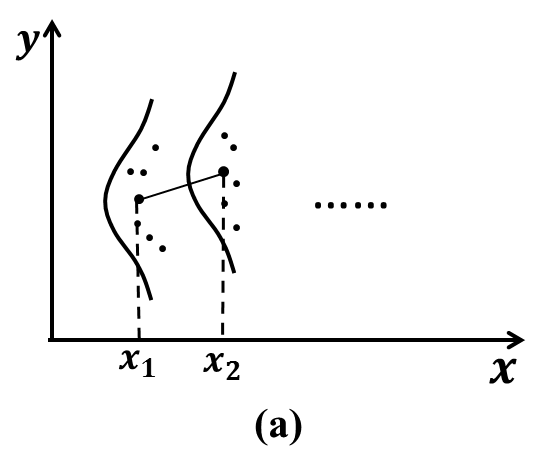
\includegraphics[height=4cm]{images/statitics_data_and_experiment_data1.jpg}
      \end{varwidth}
      \qquad \qquad
      \begin{varwidth}[t]{\textwidth}
        \vspace{0pt}
        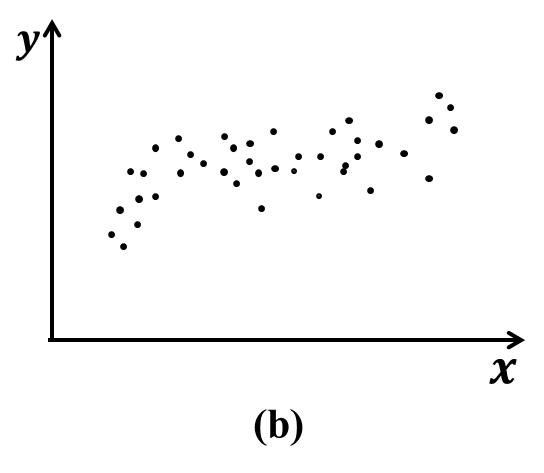
\includegraphics[height=4cm]{images/statitics_data_and_experiment_data2.jpg}
      \end{varwidth}
    \caption{统计数据和实验数据的图示}
    \label{fig:统计数据和实验数据的图示}
    \end{figure}
    \par
    我们的问题是:$y$与$x$是什么关系?即求$f$。从局部来看问题,在给定$x = x_i$时,对应的$y_i$的取值是多少?这里,记$y$的估计值为$\hat{y}$,即$\hat{y} = f(x)$。在给定$f$的具体形式之后,每给一个$x_i$,都会对应一个$\hat{y_i} = f(x_i)$。当然,估计量$\hat{y_i}$和真实数据$y_i$之间会有误差,记误差为$\varepsilon$,$\varepsilon_i$是$\hat{y_i}$和$y_i$的误差。在模型中,有时候我们并没有把模型输出写成$\hat{y}$,但是要知道,模型的输出就是真实数据$y$的估计$\hat{y}$。
\section{参数回归}
    \subsection{线性回归}
        \par
        上面简单介绍了我们要处理的问题,下面将介绍一些求解这类回归拟合问题的方法。与后面的非参数回归相比,参数回归是关系式由含参$\theta$的$y = f(x|\theta)$决定的回归模型,我们在$x_i$点对$y_i$的估计就是用$f(x_i|\theta)$进行的。而非参数回归是依据样本数据直接给出$x_i$点的$y_i$的估计值,不需要外来参数$\theta$,并且往往也不需要$y = f(x)$有具体的形式。下面,先来介绍参数回归,然后再介绍非参数回归。
        \par
        参数回归的一般形式为
        \begin{align*}
        y = f(x|\theta) + \varepsilon
        \end{align*}
        其中:$\theta$是未知参数,$f$是含参关系式,$\varepsilon$是误差项,$x,y$是一维变量,$x,y\in R$。$f$的形式有参数$\theta$确定,求$f$也即求$\theta$。
        \par
        如果假设$f$为线性的,即$f(x|\theta) = w_0+w_1 x$,则有
        \begin{align*}
        \left\{
        \begin{aligned}
        &y=w_0+w_1 x+\varepsilon\\
        &\varepsilon_i \overset{iid}{\sim} N(0,\sigma^2) \\
        &y_i|x_i \sim N(w_0+w_1 x_i,\sigma^2)
        \end{aligned}
        \right.
        \end{align*}
        \par
        这里并不对$\varepsilon$做过多的讨论,假设$\varepsilon_i \overset{iid}{\sim} N(0,\sigma^2) $,当然也可以假设$\varepsilon$服从其它分布。有关$\varepsilon$以及模型检验、参数检验和估计量性质等问题,在后面的Logistics回归中会做一些简单的介绍。如果把 $x$扩展到$p$维, $X = (x_1,x_2,\dots,x_p)^{\mathrm{T}}$,则有多元线性回归模型
        \begin{align*}
        &y = w_0+w_1x_1+w_2x_2+\dots+w_px_p +\varepsilon\\
        &\varepsilon_i \overset{iid}{\sim} N(0,\sigma^2)
        \end{align*}
        其中:$X\in R^p$,$y\in R$,$\varepsilon$为误差项。如果继续把$y\in R$扩展到$q$维,则多元线性回归模型表示为
        \begin{align*}
        \left\{
          \begin{aligned}
          &Y = A X + \varepsilon \\
          &\varepsilon \sim N(0,\Sigma)\\
          &Y |X = N(AX,\Sigma)
          \end{aligned}
        \right.
        \end{align*}
        其中:$A,X,Y,\varepsilon$皆是矩阵(向量)形式,$\varepsilon$为误差项,是一个$n\times p$维矩阵。
    \subsection{广义线性回归}
        \par
        上面建立的线性回归模型仅能解决$x,y$是线性关系的情况,而实际数据所呈现出来的趋势往往并不是线性的,如图(\ref{fig:非线性回归示意图})(a)(b)所示
\begin{figure}[H]
    \centering
    \begin{subfigure}[b]{0.35\textwidth}
        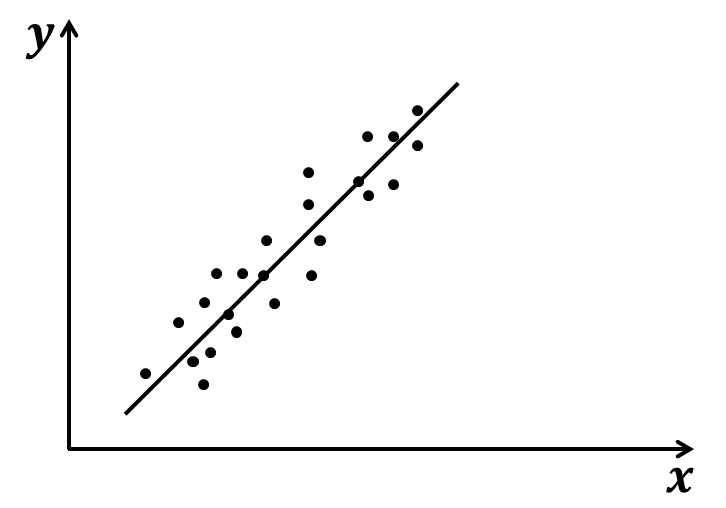
\includegraphics[width=\textwidth]{images/Non_linear_regression1.jpg}
        \caption{线性回归}
        \label{fig:线性回归}
    \end{subfigure}
    \begin{subfigure}[b]{0.35\textwidth}
        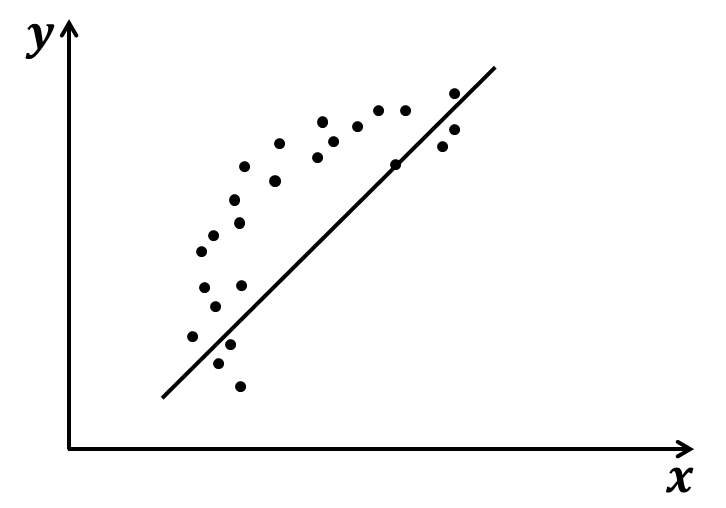
\includegraphics[width=\textwidth]{images/Non_linear_regression2.jpg}
        \caption{非线性回归}
        \label{fig:非线性回归}
    \end{subfigure}
    \caption{非线性回归示意图}\label{fig:非线性回归示意图}
\end{figure}
        为了解决图(\ref{fig:非线性回归示意图})(b)的非线性情况,我们考虑下面两种模型
        \begin{align*}
        y = ax^2+bx+c + \varepsilon\\
        y = w_0+w_1\phi(x) +\varepsilon
        \end{align*}
        \par
        第一种模型是一个二次多项式拟合模型,它要求预先给出的数据大致是2次多项式形式的,然后再对$f$中的参数$a,b,c$进行求解,这样做的缺点是:许多情况下,并不知道数据是几次的。第二种模型是一个带映射$\phi$的线性模型,由于映射$\phi$的广泛性,第二种模型可以拟合很多数据,但是此模型的难点是$\phi$的确定。由于第二种模型形式上仍然是线性的,我们称这种模型为广义线性模型,后面将主要讨论这种模型,并且假设总能预先找到合理的$\phi$。
    \subsection{参数估计}
        \par
        上面给出了线性模型和广义线性模型,模型中有参数$w = (w_1,w_2,\dots)$和$\sigma^2$是待求的,下面将介绍一些参数估计方法。考虑如下(广义)线性模型
        \begin{align}
        \label{二维广义线性模型}
        \left\{
        \begin{aligned}
        &y = w_0+w_1\phi(x)+\varepsilon \\
        &\hat{y} = w_0+w_1\phi(x)\\
        &\varepsilon_i\overset{iid}{\sim} N(0,\sigma^2)\\
        &y_i|x_i \sim N(w_0+w_1\phi(x_i),\sigma^2)
        \end{aligned}
        \right.
        \end{align}
        其中:$x,y \in R$,$\phi$为一映射。有样本数据$x_i,y_i$,样本数为$n$,模型中$w_0,w_1,\sigma$为待求参数。我们的目标是求$f$,而$f$由$w_0,w_1,\sigma$决定,所以目标变为$w_0,w_1,\sigma$的参数估计问题。记$\theta = (w_0,w_1,\sigma)$,对于求$\theta$,很自然想到:如果问题是一个优化问题就好了,我们在参数空间$\theta\in \Theta$中寻找最优参数,使得某个给定的目标最小。最终迭代得到的$\theta$即为参数$\theta$的估计值,记为$\hat{\theta}$或者$\theta^*$。
        \subsubsection{极大似然估计ML}
            在前面的模型(\ref{二维广义线性模型})中,给出了样本概率$y_i|x_i \sim N(w_0+w_1\phi(x_i),\sigma^2)$,还可以写为$y_i|x_i \sim N(\hat{y}_i,\sigma^2) = N(f(x_i),\sigma^2)$。由极大似然估计的思想(即“样本出现的概率最大”)想到,优良的$\theta$应该会使样本数据出现的概率最大。由于样本是独立同分布的,可以给出样本的联合概率密度
            \begin{align*}
            L = P\{y_1,y_2,\dots,y_n\} = \prod_{i=1}^np(y_i)
            \end{align*}
            \par
            由此可以求解$w$,使$L$最大,有
            \begin{align*}
            \max_w L(w) &= \prod_{i=1}^n p(y_i)\\
            &=\prod_{i=1}^n\frac{1}{\sqrt{2\pi \sigma^2}}e^{-\frac{(y_i - \hat{y}_i)^2}{2\sigma^2}}\\
            &=\frac{1}{(2\pi)^{\frac{n}{2}}\sigma^n} e^{-\frac{1}{2\sigma^2}(y-\hat{y})'(y-\hat{y})}
            \end{align*}
            注:已知$\phi$,给出一个$w$,则有$f(x|w)$,即$\hat{y}_i = f(x_i|w)$,从而有$y_i - \hat{y}_i$,从而有$L(w)$。这里的$\hat{y} = (\hat{y}_1,\hat{y}_2,\dots,\hat{y}_n)$。
            \par
            要求$L(w)$的最大值,由于$L(w)$与$\ln L(w)$取最大值时的$w^{*}$相同,所以$\mathop{\max}\limits_w L(w)$等价于$\max \limits_w\ln L(w)$,即上述优化问题变为
            \begin{align*}
            \max_w \ln L(w) = - n\ln (\sqrt{2\pi}\sigma) - \frac{1}{2\sigma^2}(y - \hat{y}'(y - \hat{y}))
            \end{align*}
            并且,注意到上式右边第1项与$w$无关,是常数,故优化问题变为
            \begin{align*}
            \min_w (y-\hat{y})'(y-\hat{y}) = \min_w \sum_{i=1}^n(y_i-\hat{y}_i)^2
            \end{align*}
            \par
            由极值原理
            \begin{align*}
            \frac{\partial \ln L}{\partial w} = 0
            \end{align*}
            可以求$w$。
        \subsubsection{最小二乘估计OLS}
            \par
            上面的极大似然估计(ML)的目标是求$w$,使得样本出现的概率最大,ML方法是完全基于统计思想的(在概率下使用)。下面,我们来介绍一种应用更普遍的参数估计方法 - 最小二乘法(OLS)。
            \par
            最小二乘法的目标是求$w$,使得$y$和$\hat{y}$的离差平方和最小,即
            \begin{align}
              \label{线性回归的最小二乘优化目标}
            \min_w Q(w) = \sum_{i=1}^n(y_i-\hat{y}_i)^2
            \end{align}
            其中:$\hat{y}_i= w_0+w_1\phi(x_i)$。其实,我们还可以设定其它目标,比如:求$w$使得离差绝对值的和最小;求$w$使得离差最大值最小等等
            \begin{align*}
            &\min_w \sum_{i=1}^n |y_i-\hat{y}_i|\\
            &\min_w \max_{1\leqslant i \leqslant n} |y_i - \hat{y}_i|\\
            &\min_w \sqrt[p]{\sum_{i=1}^n(y_i - \hat{y}_i)^p}
            \end{align*}
            总之,目标很关键也很灵活,并且,可以看到OLS最终的目标和ML的一样。求$Q(w)$的最小值,即$Q$对$w_0,w_1$求导,然后令导数为0,有
            \begin{align*}
            &\left\{
            \begin{aligned}
            \frac{\partial Q}{\partial w_0} = 0\\
            \frac{\partial Q}{\partial w_1} = 0
            \end{aligned}
            \right.\\
            \Rightarrow {} &
            \left\{
            \begin{aligned}
            \hat{w}_0 = \bar{y} - \hat{w}_1\bar{\phi}(x)\\
            \hat{w}_1 = \frac{\sum \phi(x_i)y_i}{\sum \phi(x_i)^2}
            \end{aligned}
            \right.
            \end{align*}
            \par
            上面的模型(\ref{二维广义线性模型})是在二维$x,y\in R$中讨论的,并且没有给出参数$\sigma$的估计(这个参数的估计应该很明了)。现在,我们将$x$推广到$p$维,考虑如下广义多元线性回归模型
            \begin{align*}
            \left\{
            \begin{aligned}
            &y = w_0 + \sum_{j=1}^{m-1}w_j \phi_j(x) +\varepsilon \\
            &\varepsilon_i \overset{iid}{\sim} N(0,\sigma^2)\\
            &y_i|x_i\sim N(\hat{y}_i,\sigma^2)
            \end{aligned}
            \right.
            \end{align*}
            将上面的模型写为矩阵的形式,有
            \begin{align*}
            y = \phi(x)w + \varepsilon
            \end{align*}
            当然也可以写为$y = w^{\mathrm{T}}\phi(x)+\varepsilon$,只是行列调换而已。其中:$m$为映射$\phi$的大小,$\phi = (\phi_1,\phi_2,\dots,\phi_m)$,$\phi(x)$是一个$n\times m$维矩阵
            \begin{align*}
            \phi(x) =
            \begin{pmatrix}
            \phi_0(x_1)&\phi_1(x_1)&\dots&\phi_{m-1}(x_1)\\
            \phi_0(x_2)&\phi_1(x_2)&\dots&\phi_{m-1}(x_2)\\
            \vdots&\vdots&\ddots&\vdots\\
            \phi_0(x_n)&\phi_1(x_n)&\dots&\phi_{m-1}(x_n)\\
            \end{pmatrix}
            _{n\times m}
            \end{align*}
            如果取特殊的$\phi$,我们可以令$m = p$,或者说每一个变量$x_j$都加一个$\phi_j$,即
            \begin{align*}
            y = w_0 + \sum_{j = 1}^p\phi_j(x_j)+\varepsilon
            \end{align*}
            \par
            我们仍然采用最小二乘来求参数$w = (w_0,w_1,\dots,w_{m-1})$,有
            \begin{align*}
            \min_w  Q(w) = \sum_{i=1}^n \varepsilon_i^2 &= \varepsilon '\varepsilon \\
            &=(y - \phi(x)w) '(y - \phi(x)w)\\
            &=||y - \phi(x)w||^2
            \end{align*}
            由极值原理,有
            \begin{align*}
            &\frac{\partial Q}{\partial w}= 0\\
            \Rightarrow {}& \frac{\partial (y - \phi(x)w) '(y - \phi(x)w)}{\partial w} = 0\\
            \Rightarrow {}& \frac{\partial(y'y - w'\phi(x)'y - y'\phi(x)w + w'\phi(x)'\phi(x)w)}{\partial w} = 0\\
            \Rightarrow {}&\frac{\partial }{\partial w}(y'y - 2y'\phi(x)w+w'\phi(x)'\phi(x)w) = 0
            \end{align*}
            即
            \begin{align*}
            -\phi(x)'y+\phi(x)'\phi(x)w = 0
            \end{align*}
            推得
            \begin{align}
            \label{权重w计算公式}
            w = (\phi(x)'\phi(x))^{-1}\phi(x)'y
            \end{align}
            注:其本质是这样的
            \begin{align*}
            &y = \phi(x)w\\
            &\phi(x)'y = \phi(x)'\phi(x)w\\
            &(\phi(x)'\phi(x))^{-1}\phi(x)'y = w
            \end{align*}

    \subsection{正则化}
        \par
        在上面求得的权重$w$计算公式(\ref{权重w计算公式})中,$w$被写为
        \begin{align*}
        w = (\phi(x)'\phi(x))^{-1}\phi(x)'y
        \end{align*}
        为简便,我们将其简略为
        \begin{align}
        \label{权重w的简写计算公式}
        w = (x^{\mathrm{T}}x)^{-1}x^{\mathrm{T}}y
        \end{align}
        \par
        对于计算公式(\ref{权重w的简写计算公式}),有两个值得讨论的地方:
        \ding{172} $x^{\mathrm{T}}x$是否可逆,即推导时$x^{\mathrm{T}}x$能除过去吗?
        \ding{173} 在$x^{\mathrm{T}}x$可逆的情况下,$(x^{\mathrm{T}}x)^{-1}$的计算量如何?可以想象,当$n$越大时,计算量越大。
        \par
        对于一个方阵$x^{\mathrm{T}}x$而言,如果行列式$|x^{\mathrm{T}}x|$不满秩,则$x^{\mathrm{T}}x$不可逆,其特征根中至少有一个是0,矩阵为奇异矩阵;如果$|x^{\mathrm{T}}x| \neq 0$,则$x^{\mathrm{T}}x$可逆,即 $(x^{\mathrm{T}}x)^{-1}$可求。
        \par
        由数据集给出的$x^{\mathrm{T}}x$肯定是可逆的,但是$x^{\mathrm{T}}x$的行列式$|x^{\mathrm{T}}x|$的值可能非常小,这导致$x^{\mathrm{T}}x$的一个很小的差异,就会引起$(x^{\mathrm{T}}x)^{-1}$很大的波动(可以想象为$\frac{1}{a}$,$a$很小,则$a$的一个微小的波动$\frac{1}{a}$都变化很大,从$y = \frac{1}{x}$的图像可以明显看出)。即当$|x^{\mathrm{T}}x| \rightarrow 0$时,$w$的估计具有不稳定性。令$A = x^{\mathrm{T}}x$,则
        \begin{align*}
        A^{-1}= \frac{1}{|A|} A^*
        \end{align*}
        其中:$A^*$是$A$的伴随矩阵。对于近似奇异的情况$|A|\rightarrow 0$,$|A|$的一个小变化会导致$\frac{1}{|A|}$巨大的变化,从而$A^{-1}$变化巨大。对于这种近似奇异的情况,我们只要将$|A|$调大一些就好了,由于$|A|\rightarrow 0$时,$|A| = \prod_{i=1}^n\lambda_i$,不妨将$A$修正为
        \begin{align*}
        A := A+\lambda I
        \end{align*}
        其中:$\lambda$为常参数,$I$为单位矩阵。
        \par
        由上面的修正思想,我们可以得到如下的$w$的修正计算公式
        \begin{align}
        \label{权重w修正计算公式}
        w = (x^{\mathrm{T}}x + \lambda I)^{-1}x^{\mathrm{T}}y
        \end{align}
        其中:$\lambda$为turning parameter。与(\ref{权重w修正计算公式})式对应的最小二乘优化问题为岭回归(ridge regression)
        \begin{align*}
        \min_w\ Q(w) &= ||y - x w||^2 + \lambda ||w||^2\\
        &= \sum_{i=1}^n(y_i-\hat{y}_i)^2+\lambda\sum_{j = 0}^m w_j^2
        \end{align*}
        我们称$||w||^2$项为正则项(罚项)。上面岭回归的正则项是二次的,当然我们可以用其它的形式,比如lasso regression中用的一次罚项(1996.Tibshirami)
        \begin{align*}
        \min_w \ Q(w) = ||y  - wx||^2+\lambda||w||^1
        \end{align*}
        其中:$||w||^1 =\sum_{j=1}^m |w_j|$。但是,lasso并不能像岭回归和普通线性回归那样写出显式的$w$的计算公式。更一般的,我们还可以写出正则项为$\lambda||w||^p$时的最小二乘优化目标
        \begin{align*}
        \min_w \ Q(w) = ||y-\hat{y}||^2 + ||w||^p
        \end{align*}
        \par
        我们来观察一下不同$p$时,正则项的轮廓线图,如图(\ref{fig:正则项的轮廓线})所示
        \begin{figure}[H]
          \centering
          \begin{varwidth}[t]{\textwidth}
            \vspace{0pt}
            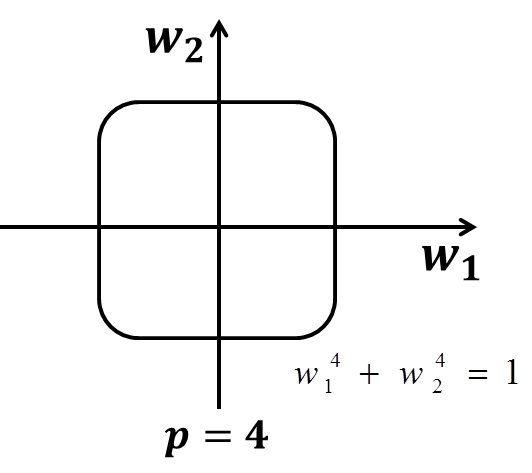
\includegraphics[height=4cm]{images/The_contour_of_regular_term1.jpg}
          \end{varwidth}
          \begin{varwidth}[t]{\textwidth}
            \vspace{0pt}
            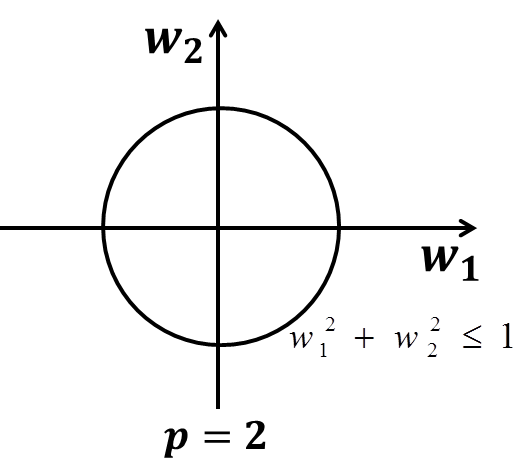
\includegraphics[height=4cm]{images/The_contour_of_regular_term2.jpg}
          \end{varwidth}
          \begin{varwidth}[t]{\textwidth}
            \vspace{0pt}
            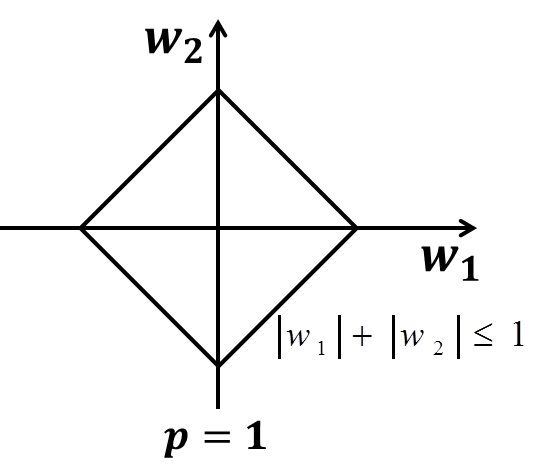
\includegraphics[height=4cm]{images/The_contour_of_regular_term3.jpg}
          \end{varwidth}
            \begin{varwidth}[t]{\textwidth}
            \vspace{0pt}
            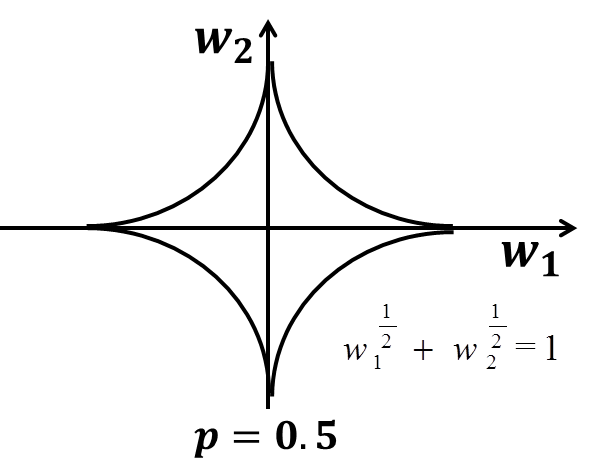
\includegraphics[height=4cm]{images/The_contour_of_regular_term4.jpg}
          \end{varwidth}
            \begin{varwidth}[t]{\textwidth}
            \vspace{0pt}
            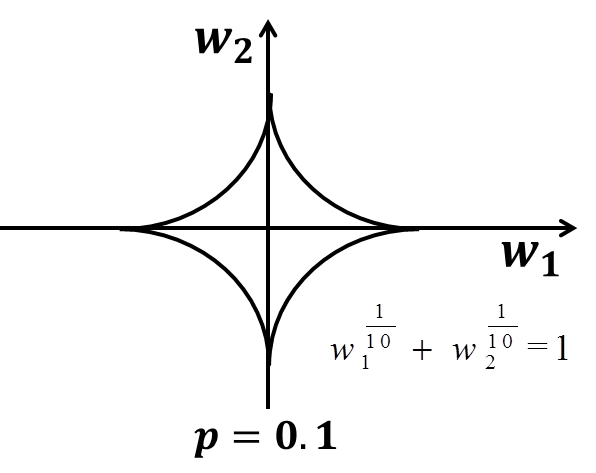
\includegraphics[height=4cm]{images/The_contour_of_regular_term5.jpg}
          \end{varwidth}
        \caption{正则项的轮廓线}
        \label{fig:正则项的轮廓线}
        \end{figure}
        % \textcolor[rgb]{1 0 0}{todo:matlab图片:正则项的轮廓线}\\
        一般情况下,最好令$p \geqslant 1$,因为当$p <1$时,集合变为非凸,从而优化问题也变为一个非凸优化。
        \par
        上面是在$x$上讨论的,我们将$x$还原为$\phi(x)$。当$p=2$时,$\phi(x)$对应的岭回归的最小二乘优化目标为
        \begin{align}
        \label{ridge回归的一般形式}
        \min_w \ Q(w) &= \frac{1}{2}||y - \hat{y}||^2+\frac{1}{2}\lambda||w||^2\notag\\
        &=\frac{1}{2}\sum_{i=1}^n(y_i - \phi(x_i)w)^2 + \frac{1}{2}\lambda w^\mathrm{T}w
        \end{align}
        其$w$计算公式为
        \begin{align*}
        w = (\phi^\mathrm{T}(x)\phi(x)+\lambda I)^{-1} \phi^\mathrm{T}(x)y
        \end{align*}
        \par
        当$p = 1$时,$\phi(x)$对应的lasso regression的最小二乘优化目标为
        \begin{align}
        \label{lasso回归的一般形式}
        \min_w\ Q(w) = \frac{1}{2}\sum_{i=1}^n(y_i - \phi(x_i)w)^2+\frac{1}{2}\lambda\sum_{j=1}^m|w_j|
        \end{align}
        如果$\lambda$很大,那么某些$w_j$就会变为0,从而产生稀疏(Spase)模型。值得一提的是,当$\phi^\mathrm{T}\phi$接近奇异时,可以通过奇异值分解(SVD)来解决这一问题,并且记$\phi^{\dagger} = (\phi^\mathrm{T}\phi)^{-1}\phi^{\mathrm{T}}$是矩阵$\phi$的Moore-Penrose伪逆矩阵。关于ridge和lasso我们后面还会介绍。
    \subsection{随机梯度下降算法及其变体}
        \par
        上面建立的回归模型如:广义线性回归(\ref{线性回归的最小二乘优化目标})、岭回归(\ref{ridge回归的一般形式})和lasso回归(\ref{lasso回归的一般形式})都有相应的优化算法。我们写出最小二乘问题一般形式
        \begin{align}
        \label{最小二乘问题的一般形式}
        \min_\theta \ J(\theta) = \frac 1n f_i(\theta)
        \end{align}
        其中:$f_i$就相当于最小二乘中的$(y_i - \hat{y}_i(w))^2$,我们称其为样本点$(x_i,y_i)$的损失函数。注意:这里的一般形式(\ref{最小二乘问题的一般形式})并没有包含正则化项。MATLAB最优化工具箱使用两种算法来求解有约束线性最小二乘问题:
        \begin{enumerate}
        \item 有效集算法用于求解有边界的问题以及线性不等式或等式。
        \item 信赖域反射用于求解只带有边界约束的大规模问题。
        \end{enumerate}
        该工具箱使用两种算法来求解非线性最小二乘问题:
        \begin{enumerate}
        \item 信赖域反射算法采用信赖域方法来实现 Levenberg-Marquardt 算法。它用于无约束和有边界约束的问题。
        \item Levenberg-Marquardt 算法实现标准的 Levenberg-Marquardt 算法。它用于无约束问题。
        \end{enumerate}
        MATLAB求解最小二乘优化问题的命令为lsqcurvefit,应用示例
        \begin{lstlisting}[language = Matlab]
        x = Data(:,1);y = Data(:,2);
        F = @(w,xdata)w(1)*exp(-w(2)*xdata) + w(3)*exp(-w(4)*xdata);
        w0 = [1 1 1 0];
        [w,resnorm,~,exitflag,output] = lsqcurvefit(F,w0,x,y)
        plot(x,y,'ro'),hold on
        plot(x,F(w,x)),hold off
        title('非线性最小二乘')
        \end{lstlisting}
        关于最小二乘优化问题的一般性解法,可以参考最优化部分相应的章节。lsqcurvefit采用的方法都是确定性算法:每一迭代步长是多少,迭代方向是哪里,都是完全确定的。下面,我们来介绍机器学习模型中常用的优化方法 - 随机梯度下降方法及其变体,这种方法具有随机性,可以跳出局部极小值点。
        \par
        为了和一般的参考文献统一,我们将最小二乘模型中的符号变为下列形式
        \begin{align*}
        J(\theta) = \frac{1}{2n}\sum_{i=1}^n \left(y^{(i)}  -  h_\theta \left( x^{(i)} \right) \right) ^2
        \end{align*}
        其中:$y^{(i)}$为第$i$个样本的因变量$y$值,$x^{(i)}$为第$i$个样本的自变量$x$值,由于有$p$个自变量$x_i$,所以$x^{(i)} = (x_1^{(i)},x_2^{(i)},\dots,x_p^{(i)}) \in R^p$,$h_\theta \left( x^{(i)} \right) $为
        \begin{align*}
        h_\theta \left( x^{(i)} \right)  = \sum_{j = 1}^p\theta_j x_j^{(i)}
        \end{align*}
        \subsubsection{梯度下降算法GD}
            \par
            Gradient Descent:在更新每一个参数$\theta_j,j = 1,\dots,p$时,都使用所有样本,则有$\theta_j$的梯度方向
            \begin{align*}
            \nabla \theta_j = \frac{\partial J}{\partial \theta_j} = -\frac{1}{n}\sum_{i=1}^n\left(y^{(i)}  -  h_\theta \left( x^{(i)} \right) \right) x_j^{(i)}
            \end{align*}
            于是,参数更新公式为
            \begin{align*}
            \theta_j \leftarrow : \theta_j - \eta \nabla \theta_j
            \end{align*}
            其中:$\eta$为学习率,可以是变化的学习率$\eta_t$。由此算法得到的$\theta$是一个全局最优解,但是每一步都要用到所有的样本数据(训练集),当$n$很大时,效率非常低。记$\nabla _\theta J(\theta)$为$J$关于$\theta$的梯度。
        \subsubsection{随机梯度下降算法SGD}
            \par
            Stochastic Gradient Descent:每次迭代使用一个样本,并用次样本来更新所有参数$\theta_j(j = 1,\dots,p)$,有$\theta_j$的梯度方向
            \begin{align*}
            \nabla \theta_j = \left(y^{(i)}  -  h_\theta \left( x^{(i)} \right) \right) x_j^{(i)}
            \end{align*}
            \par
            SGD伪代码如下(\ref{code:SGD})
            \begin{algorithm}[h]
                \caption{随机梯度下降SGD}\label{code:SGD}
                \begin{algorithmic}[1]
                    \Require 样本数据$(x^{(i)},y^{(i)})_{i=1}^n$,$x^{(i)}\in R^p,y^{(i)}\in R$,学习率$\eta$
                    \Ensure 参数$\theta$
                    \For{$i = 1,2,\dots,n$}
                      \For{$j = 1,2,\dots,p$}
                        \State $\nabla \theta_j = \left(y^{(i)}  -  h_\theta \left( x^{(i)} \right) \right) x_j^{(i)}$
                        \State $\theta_j \leftarrow:\theta_j - \eta \nabla\theta_j$
                      \EndFor
                      \State $//$ 或者写为向量形式
                      \State $\theta \leftarrow: \theta - \eta \nabla_\theta J(\theta;x_i,y_i)$
                    \EndFor
                \end{algorithmic}
            \end{algorithm}
            \par
            值得注意的是SGD得到的$\theta$并不是全局最优解,并且每次$\theta_j$下降的方向也不是全局梯度下降方向,它的下降方向只是使某一样本$x_i,y_i$的离差平方$(\hat{y}_i - y_i)^2$最小。由于这种异步操作,SGD并不易于并行实现,但其收敛速度快,并且,从另一个角度来看,非全局梯度下降有利于跳出局部极小解,因此,SGD在非凸优化中也表现突出(如:神经网络和深度网络等)。
        \subsubsection{小批量梯度下降算法MBGD}
            \par
            上面的梯度下降算法GD每次迭代使用所有样本,随机梯度下降算法SGD每次迭代使用一个样本,自然地,我们想到一次使用部分样本,我们称这种一次迭代使用部分样本的算法为小批量随机梯度下降算法(Mini-Batch Gradient Descent)。每次随机的从样本$n$中挑取$b$个样本,这里的$b$即为批量的大小,用着$b$个样本来更新$\theta$,有$\theta_j$的梯度方向为
            \begin{align*}
            \nabla \theta_j = \frac{1}{b} \sum_{i=1}^b\left(y^{(i)}  -  h_\theta \left( x^{(i)} \right) \right) x_j^{(i)}
            \end{align*}
            \par
            MBGD伪代码如下(\ref{code:MBGD})
            \begin{algorithm}[h]
                \caption{小批量梯度下降算法MBGD}\label{code:MBGD}
                \begin{algorithmic}[1]
                    \Require 样本数据$(x^{(i)},y^{(i)})_{i=1}^n$,$x^{(i)}\in R^p,y^{(i)}\in R$,学习率$\eta$,批量大小$b$,迭代次数$t$,最大迭代次数$T$
                    \Ensure 参数$\theta$
                    \For{$t = 1,2,\dots,T$}
                      \State 从样本$n$中挑取$b$个样本$x_t,y_t$
                      \For{$j = 1,2,\dots,p$}
                        \State $\nabla \theta_j = \frac{1}{b} \sum\limits_{i=1}^b\left(y^{(i)}  -  h_\theta \left( x^{(i)} \right) \right) x_j^{(i)}$
                        \State $\theta_j \leftarrow:\theta_j - \eta \nabla\theta_j$
                      \EndFor
                      \State $//$ 或者写为向量形式
                      \State $\theta \leftarrow: \theta - \eta \nabla_\theta J(\theta;x_{t},y_{t})$
                    \EndFor
                \end{algorithmic}
            \end{algorithm}
            \par
            可以发现,MBGD是BGD和GD的综合,相对于SGD,MBGD降低了随机性带来的波动,使更新更加稳健;相对于BGD,MBGD提高了收敛速率,同时随机性有助于跳出局部极小值,因此更多时候,我们采用MBGD算法。但如SGD那样,MBGD的更新方向不是全局梯度方向,其解亦非全局最优解。
            \par
            从收敛速度来看,SGD能够在目标函数是强凸且递减学习率的情况下,以$O(\frac{1}{T})$次线性收敛,而GD以$O(\rho^T)(\rho<1)$线性收敛,其中:$T$为迭代总次数。
        \subsubsection{动量因子法Momentum}
            \par
            动量因子法是模拟物理中动量的概念,用累计的动量来替代梯度,可以参考1999.Qian\cite{1999.Qian}。动量项为
            \begin{align*}
            v_t = rv_{t-1}+\eta \nabla \theta
            \end{align*}
            其中:$\nabla \theta = (\nabla \theta_1,\dots,\nabla\theta_j,\dots,\nabla\theta_p)$,动量项超参数$r<1$,一般情况取0.9以下。参数更新为
            \begin{align*}
            \theta \leftarrow: \theta - v_t
            \end{align*}
            \par
            在更新参数时,如果当前$\theta_j$的梯度方向与上次梯度方向相同,则$\theta_j$在这个方向上的更新会更快,当达到局部极小值附近时,$\nabla\rightarrow 0$,$r$使得更新幅度增大,从而可以跳出局部解。
        \subsubsection{NAG}
            1983.Nesterov\cite{1983.Nesterov}提出Nesterov accelerated gradient,NAG不仅增加了动量项,并且在计算参数的梯度时,从损失函数$J(\theta)$中减去了动量项
            \begin{align*}
            v_t = r v_{t-1} + \eta \nabla_\theta J(\theta - r v_{t-1})
            \end{align*}
            $\theta$的更新公式为
            \begin{align*}
            \theta \leftarrow :\theta - v_t
            \end{align*}
            \par
            其实,momentum和nesterov项都是为了使梯度更加灵活,但是人工设置学习率还是有些主观,接下来介绍几种自适应学习算法。
        \subsubsection{Adagrad}
            2011.Duchi,Hazan和Singer\cite{2011.Duchi}提出Adagrad算法。前面介绍的所有算法,它们在每次更新参数时,对所有参数$\theta_i,\dots,\theta_p$都使用相同的学习率$\eta$,如果数据是稀疏的,或者每个特征$x_j$有着不同的统计特征,那么,便不能使用相同的学习率。那些很少出现的特征应该使用一个较大的学习率。
            \par
            Adagrad能够对每个参数$\theta_j$自适应一个学习率$\eta_t^j$,对稀疏特征,得到一个大的学习率,因此,该Adagrad算法适合处理有稀疏特征的数据。令参数梯度为
            \begin{align*}
            \nabla\theta_j = \nabla_\theta J(\theta_j)
            \end{align*}
            则参数$\theta_j$的Adagrad更新公式为
            \begin{align*}
            \theta_j\leftarrow : \theta_j - \eta\frac{1}{\sqrt{G_{t,j}+\epsilon}}\nabla\theta_j
            \end{align*}
            其中:$G_t\in R^{p\times p}$是一个对角矩阵,其第$j$个对角元素$e_{jj}$为过去到当前第$j$个参数$\theta_j$的梯度平方和,即
            \begin{align*}
            e_{jj} \leftarrow: e_{jj} + \nabla \theta_j^2
            \end{align*}
            $\epsilon$是为了使分母不为0,通常取$1e-8$。另外,如果分母不开根号,算法的性能会非常糟糕。上式的向量形式为
            \begin{align*}
            \theta \leftarrow :\theta - \eta \frac{1}{\sqrt{G_t+\epsilon}} \cdot \nabla \theta
            \end{align*}
        \subsubsection{Adadelta}
            虽然Adagrad能够自适应学习率,但其仍然依赖于人工设置的全局学习率$\eta$,并且Adagrad还需要计算参数梯度序列平方和$e_{jj}$,这会使存储量增加,此外,学习率是不断衰减的,最终达到一个非常小的值。为了克服Adagrad的这个缺点,2012.Zeiler\cite{2012.Zeiler}提出了Adadelta算法,令
            \begin{align*}
            g_t = \nabla _\theta J(\theta)
            \end{align*}
            其中:$t$表示迭代次数。计算梯度平方的期望然后累加
            \begin{align*}
            E|g^2|_t = E|g^2|_{t-1}+(1-\gamma) g_t^2
            \end{align*}
            计算参数更新量
            \begin{align*}
            \Delta \theta_t = \frac{\sqrt{\sum_{r = 1}^{t-1}\nabla \theta_r}}{\sqrt{E|g^2|_t+\epsilon}}
            \end{align*}
            最终,有参数更新公式
            \begin{align*}
            \theta_{t+1}\leftarrow:\theta_t -\Delta\theta_t
            \end{align*}
            \par
            注意,此时$\theta$的更新已经不再依赖于全局学习率了。
        \subsubsection{RMSprop}
            \par
            RMSprop是Adadelte的中间形式
            \begin{align*}
            E|g^2|_t = \gamma E|g^2|_{t-1}+ (1-\gamma)g_t^2\\
            \Delta \theta_t =\eta \frac{1}{\sqrt{E|g^2|_t + \epsilon}}\cdot g_t
            \end{align*}
            $\theta$的更新公式为
            \begin{align*}
            \theta_{t+1} \leftarrow :\theta_t - \eta \Delta \theta_t
            \end{align*}
            \par
            在深度学习模型中,Hinton建议将参数设置为$r = 0.9,\eta = 0.01$。
        \subsubsection{Adam}
            \par
            Adam(Adaptive Moment Estimation)利用梯度的一阶矩估计和二阶矩估计动态调整每个参数的学习率
            \begin{align*}
            &v_t = \beta_1(v_{t-1})+(1-\beta_1)g_t\\
            &n_t = \beta_2(n_{t-1})+(1-\beta_2)g_t^2\\
            &\hat{v}_t = \frac{v_t}{1-\beta_1^t}\\
            &\hat{n}_t = \frac{n_t}{1-\beta_2^t}\\
            &\Delta \theta_t = \eta \frac{\hat{v}_t}{\sqrt{\hat{n}_t}+\epsilon}
            \end{align*}
            最终,$\theta$的更新公式为
            \begin{align*}
            \theta_{t+1} \leftarrow:\theta_t - \Delta \theta_t
            \end{align*}
        \par
        上面介绍了随机梯度下降算法及其变体,我们引入两幅经典的图\footnote{http://sebastianruder.com/optimizing-gradient-descent/?url\_type=39\&object\_type=webpage\&pos=1}(\ref{fig:随机梯度下降算法及其变体的比较})来比较随机梯度下降算法及其变体
           \begin{figure}[H]
               \centering
               \begin{subfigure}[b]{0.4\textwidth}
                   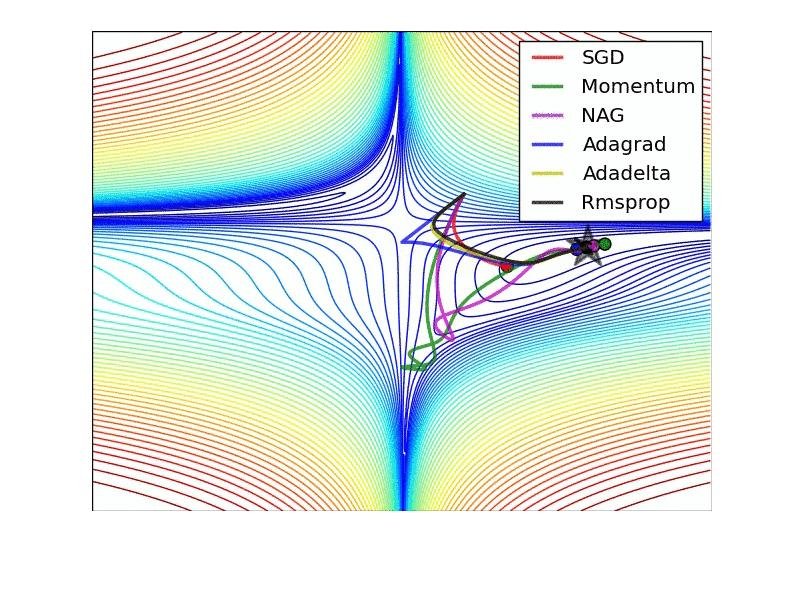
\includegraphics[width=\textwidth]{images/compare_stochastic1.jpg}
                   \caption{}
                   \label{fig:图1}
               \end{subfigure}
               \begin{subfigure}[b]{0.4\textwidth}
                   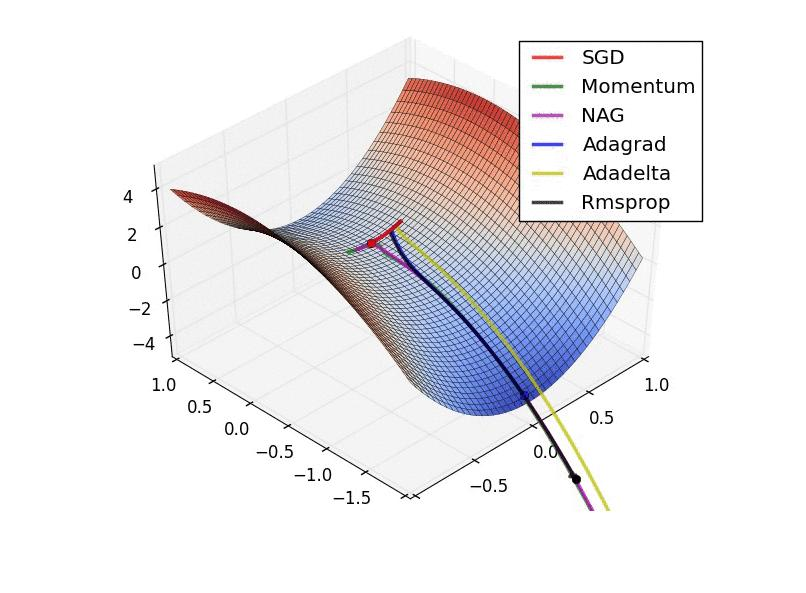
\includegraphics[width=\textwidth]{images/compare_stochastic2.jpg}
                   \caption{}
                   \label{fig:图2}
               \end{subfigure}
               \caption{随机梯度下降算法及其变体的比较}
               \label{fig:随机梯度下降算法及其变体的比较}
           \end{figure}
% 添加动态图gif
% \usepackage{animate}
% \begin{document}
% \begin{frame}
%   \animategraphics[
%   autoplay,loop,controls,
%   width=.7\textwidth,
%   height=.7\textheight
%   ]{4}{ra-}{0}{3}
% \end{frame}
% \end{document}
% controls代表添加手动控制按钮,4代表一秒播放几张图片,ra-代表循环播放的PNG图片名前缀,0和3代表播放的第一张图片和最后一张图片的序号。
        从图(\ref{fig:随机梯度下降算法及其变体的比较})中我们可以看出,在优化问题的鞍点处(saddle points:某些维度上梯度为0,某些不为0),SGD、Momentum和NAG一直在鞍点梯度为0的方向上震荡,很难打破鞍点位置的对称性;Adagrad、Adadelta和RMSprop等能够很快的向梯度不为0的方向上移动,并且,这些自适应学习方法有更好的收敛性和收敛速度。
        \par
        前面,我们提到过SGD是次线性收敛的,而GD是线性收敛的,那么能否改进SGD,使SGD能够达到线性收敛速度?有的,下面我们来介绍SAG和SVRG。
        \subsubsection{SAG}
            \par
            SAG的伪代码如下(\ref{code:SAG})
            \begin{algorithm}[h]
                \caption{Basic SAG method for minimizing $J(\theta) = \frac 1n \sum_{i = 1}^nf_i(\theta)$with step size $\eta$}\label{code:SAG}
                \begin{algorithmic}[1]
                    \Require 样本数据$(x^{(i)},y^{(i)})_{i=1}^n$,$x^{(i)}\in R^p,y^{(i)}\in R$,学习率$\eta$,迭代次数$t$,最大迭代次数$T$
                    \Ensure 参数$\theta$
                    \State 初始化。$d= 0,g_i = 0$
                    \For{$t = 1,2,\dots,T$}
                      \State 从样本$n$中挑取1个样本$x^{(i)},y^{(i)}$
                      \For{$j = 1,2,\dots,p$}
                        \State $d_j = d_j - g_i^j + \nabla _\theta J(\theta_j|x^{(i)},y^{(i)})$
                        \State $g_i^j = \nabla _\theta J(\theta_j|x^{(i)},y^{(i)})$
                        \State $\theta_j \leftarrow:\theta_j - \frac{\eta}{n} d_j$
                      \EndFor
                      \State $//$ 或者写为向量形式
                      \State $d = d - g_i + \nabla _\theta J_i(\theta)$
                      \State $g_i = \nabla_\theta J_i(\theta)$
                      \State $\theta \leftarrow :\theta - \frac{\eta}{n}d$
                    \EndFor
                \end{algorithmic}
            \end{algorithm}
            \par
            SAG为每一个样本$(x_i,y_i)$(伪代码中写为$x^{(i)},y^{(i)}$)都维护了一个梯度$g_i$,随机选择一个样本$x_i,y_i$来更新$d$,并用$d$来更新参数$\theta$。
        \subsubsection{SVRG}
            \par
            SVGR的伪代码如下(\ref{code:SVRG})
            \begin{algorithm}[h]
                \caption{Basic SVRG method for minimizing $J(\theta) = \frac 1n \sum_{i = 1}^nf_i(\theta)$with step size $\eta$}\label{code:SVRG}
                \begin{algorithmic}[h]
                    \Require 样本数据$(x^{(i)},y^{(i)})_{i=1}^n$,$x^{(i)}\in R^p,y^{(i)}\in R$,学习率$\eta$,迭代次数$t$,最大迭代次数$T$
                    \Ensure 参数$\theta$
                    \State 初始化:$\tilde{\theta}_0 $
                    \For{$t = 1,2,\dots,T$}
                      \State $\tilde{\theta} \leftarrow \tilde{\theta}_{t-1}$
                      \State $\tilde{g} = \frac{1}{n} \sum\limits_{i =1}^n \nabla f_i(\tilde{\theta})$
                      \State 从样本$n$中挑取1个样本$x^{(i)},y^{(i)}$
                      \For{$j = 1,2,\dots,p$,$p \equiv m$}
                        \State $d_j = d_j - g_i^j + \nabla _\theta J(\theta_j|x^{(i)},y^{(i)})$
                        \State $\Delta \theta_j = \eta \left( \nabla_\theta J_i(\theta_{j-1})  - \nabla_\theta J_i(\tilde{\theta}) + \tilde{g}\right) $
                        \State $\theta_j \leftarrow:\theta_j - \Delta \theta_j$
                      \EndFor
                      \State option 1: set $\tilde{\theta}_t = \tilde{\theta}_p$
                      \State option 2: set $\tilde{\theta}_t = \tilde{\theta}_j$,for randomly chose $j\in \{0,1,\dots,p-1\}$
                    \EndFor
                \end{algorithmic}
            \end{algorithm}
            \par
            SVRG的思路是:每隔一段时间计算一次所有样本的梯度$\tilde{g}$,每个阶段内部的单次更新采用$\nabla_\theta J_i(\theta_{j-1})  - \nabla_\theta J_i(\tilde{\theta}) + \tilde{g}$来更新参数$\theta$。SVRG每次更新最多计算两次梯度,相对SAG而言,不需要在内存中为每个样本维护一个梯度,从而节省了内存。

\section{贝叶斯回归模型}
    \par
    前面介绍了参数回归的线性回归、参数估计方法、正则回归以及随机梯度下降优化算法,下面,我们在贝叶斯框架下讨论回归模型的参数估计问题,称基于贝叶斯方法的(广义)线性回归模型为贝叶斯线性回归。
    \subsection{贝叶斯统计基础}
        \par
        在概率论中,一直存在两大学派:频率学派和贝叶斯学派。就参数估计问题而言,频率学派认为参数$\theta$是未知待求的固定量,而贝叶斯学派认为参数$\theta$是随机变量,因此,Bayes的参数会存在分布。称在没给出样本前得到的分布为先验分布,先验分布是由经验积累得到的信息,如:一个企业家认为“一项新产品在未来市场上的畅销”的概率为0.8,这里的0.8就是企业家根据自己多年的经验得到的结论,即先验概率,但是后期是否真的为0.8,还需要结合实际抽样来下结论。
        \par
        为了便于叙述贝叶斯参数估计,我们先来简单介绍一下贝叶斯公式。设$A,B$和$A_i$是事件,$P(A)$为事件$A$发生的概率,$P(B|A_i)$表示$A_i$发生导致$B$发生的概率,并假设可以导致$B$发生的事件有$A_1,A_2,\dots,A_i,\dots$,有如下条件概率公式
        \begin{align*}
        &P(A|B) = \frac{P(AB)}{P(B)}\\
        &P(A_iB) = P(B)P(A_i|B) = P(A_i)P(B|A_i)
        \end{align*}
        由此,可以得到离散形式的贝叶斯公式
        \begin{align}
        \label{贝叶斯公式}
        P(A_i|B) &= \frac{P(A_i)P(B|A_i)}{P(B)} \notag\\
        &= \frac{P(A_i)P(B|A_i)}{\sum_iP(A_i)P(B|A_i)}
        \end{align}
        \par
        通俗的说,贝叶斯公式的概率意义是:事件$B$发生了,事件$B$发生是由事件$A_i$引起的概率等于$A_i$发生且$A_i$发生导致$B$发生的概率除上所有可能导致$B$发生的情况。
        \par
        贝叶斯学派认为未知待求参数是随机的,有一定的分布。我们令$\theta$为未知参数,记其先验概率为$\pi(\theta)$,令$x\in R^p$为变量,$\mathbf{x} = (x_1,\dots,x_n)$为样本,则样本$\mathbf{x}$的联合概率密度函数是在$\theta$给定下的条件密度,故$\mathbf{x}$的密度函数为$p(x|\theta)$,这里将$\theta$视为导致样本$\mathbf{x}$出现的原因,相当于$A$。由上面的贝叶斯公式(\ref{贝叶斯公式}),我们有$\theta$的后验分布
        \begin{align}
        \label{参数的后验分布}
        \pi(\theta|\mathbf{x}) = \frac{p(\mathbf{x}|\theta)\pi(\theta)}{\int_\Theta p(\mathbf{x}|\theta)\pi (\theta) \mathrm{d}\theta} = \frac{p(\mathbf{x}|\theta)\pi(\theta)}{p(\mathbf{x})}
        \end{align}
        其中:$\pi(\theta|\mathbf{x})$就是在样本$\mathbf{x}$给定后,$\theta$的后验概率,我们要求使得$\pi(\theta|\mathbf{x})$最大的$\theta^*$,这样的参数估计方法称为最大后验概率方法。
        \begin{align*}
        \max _\theta \ \pi(\theta|\mathbf{x})
        \end{align*}
        由于式(\ref{参数的后验分布})分母中的样本联合概率分布$p(\mathbf{x})$相对于$\theta$独立,故
        \begin{align*}
        \max _\theta \ \pi(\theta|\mathbf{x}) = \max_\theta p(\mathbf{x}|\theta)\pi(\theta)
        \end{align*}
        \par
        注意:这里的$p(x|\theta)$和极大似然估计中的$p(\mathbf{x};\theta)$是一样。一般而言,我们并没有任何辅助信息来确定先验概率密度$\pi(\theta)$,所以$\pi(\theta)$是主观意义上的,可以取正态分布,Gamma分布族等等。思考:如果按照贝叶斯统计的思想,我们给定参数$\theta$的带参数先验分布$\pi(\theta|\alpha,\beta)$,那么$\alpha,\beta$也是随机变量,也会有相应的先验分布和后验分布,如此下去,以致无穷,我们称$\alpha,\beta$为超参数,后面会介绍这种“无穷”问题的处理方法。
    \subsection{贝叶斯线性回归模型}
        \par
        在前面的线性回归模型中,我们假设$\varepsilon_i \overset{iid}{\sim}N(0,\sigma^2)$,$y_i|x_i\overset{iid}{\sim}N(\hat{y}_i,\sigma^2)$。并且,已经有了在参数$\theta = (w,\sigma^2),w\in R^m,\sigma\in R$给定下样本的联合概率密度
        \begin{align*}
        p(y|x,w,\beta) = \prod_{i=1}^nN(w^\mathrm{T}\phi(x_i),\beta^{-1})
        \end{align*}
        其中:$\beta = (\sigma^2)^{-1}$。此联合概率分布可以记为$p(y|\theta)$,即前面说的$p(\mathbf{x}|\theta)$,那么,根据贝叶斯公式(\ref{贝叶斯公式}),$\theta$的后验概率$\pi(\theta|y)$为
        \begin{align*}
        \pi(\theta|y) = \frac{p(y|\theta)\pi(\theta)}{\int_\Theta p(y|\theta)\pi(\theta)\mathrm{d}\theta}
        \end{align*}
        \par
        我们的目标是求$\theta$,使得后验概率$\pi(\theta|y)$最大,但还没有给出先验分布$\pi(\theta)$。下面就来讨论$\pi(\theta)$。给出参数$w$的先验概率分布,在这期间,把$\beta$当作已知常数,假设1:$w = (w_1,w_2,\dots,w_p)$的$w_i$是独立同分布的($p \equiv m$),或者说它们的先验分布是一样的;假设2:$w_i\sim N(0,\alpha^{-1})$,其中:$\alpha$为超参数。
        \par
        由各参数$w_i$先验分布一样,为正态分布$N(0,\alpha^{-1})$,我们有
        \begin{align*}
        &p(w_i;\alpha) = N(0,\alpha^{-1})\\
        &\pi(w) = \pi(w;\alpha) = N(0,\alpha^{-1}I)
        \end{align*}
        这里的$\pi(w;\alpha)$也可以记为$\pi(w|\alpha)$,表示分布$\pi(w)$是由参数$\alpha$控制的。给出了先验$\pi(w|\alpha)$之后,还要计算样本条件密度函数$p(y|\theta)$以及后验概率密度$\pi(\theta|y)$。$p(y|\theta)$即为样本的条件联合概率密度,而对于$\pi(\theta|y)$的求解,更详细的推导可以参考:《高等数理统计(第二版)》茆诗松P350例5.26或者《PRML》P67-P69。下面,我们用一示例来展示后验分布$\pi(\theta|y)$为正态分布。
        \begin{example}[正态均值的共轭先验分布为正态分布]
        \par
        我们用此示例来展示:在方差已知的情况下,正态均值的共轭先验分布为正态分布。设$y = (y_1,y_2,\dots,y_n)$是来自正态分布$N(\theta,\beta^{-1})$的样本(已知,$y$是来自$N(w^\mathrm{T}\phi(x),\beta^{-1})$的样本,而$w$就是$\theta$),其中$\beta^{-1} = \sigma^2$已知,且设参数(均值)$\theta$的先验分布为正态分布$\theta\sim N(\mu,\tau^2)$,即
        \begin{align*}
        \pi(\theta) = \frac{1}{\sqrt{2\pi}\tau}e^{-\frac{(\theta-\mu)^2}{2\tau^2}}
        \end{align*}
        其中:$\mu,\tau$已知。由此,可以写出样本$y$与$\theta$的联合密度函数
        \begin{align*}
        h(y,\theta) = k_1\exp\left\{ -\frac{1}{2}\left[ \frac{n\theta^2-2n\theta\bar{y} + \sum\limits_{i=1}^n y_i^2 }{\sigma^2}  +\frac{\theta^2-2\mu\theta + \mu^2}{\tau^2} \right] \right\}
        \end{align*}
        其中:$k_1 = (2\pi)^{-\frac{n+1}{2}} \tau^{-1}\sigma^{-n}$,$\bar{y} = E(y)$。再记
        \begin{align*}
        \sigma_0^2 = \frac{\sigma^2}{n},\quad A = \frac{1}{\sigma_0^2}+ \frac{1}{\tau^2},\quad B = \frac{\bar{y}}{\sigma_0^2}+\frac{\mu}{\tau^2},\quad C = \frac{\sum_{i=1}^n y_i^2}{\sigma^2}+ \frac{\mu^2}{\tau^2}
        \end{align*}
        则有
        \begin{align}
        \label{ytheta联合分布}
        h(y,\theta) &= k_1\left\{ -\frac{1}{2}[A\theta^2 - 2\theta B + c] \right\}\notag\\
        &=k_1\exp \left\{ -\frac{(\theta-B/A)^2}{2/A} - \frac{1}{2}(C-B^2/A) \right\}
        \end{align}
        容易计算样本$y$的边缘分布为
        \begin{align}
        \label{y的边缘分布}
        m(y) &=\int_{-\infty}^\infty h(y,\theta)\mathrm{d}\theta\notag \\
        &= k_1\exp\left\{-\frac{C-B^2/A}{2}\right\} \left( \frac{2\pi}{A} \right)^{\frac{1}{2}}
        \end{align}
        上式(\ref{ytheta联合分布})和(\ref{y的边缘分布})相除,可以得到$\theta$的后验分布
        \begin{align*}
        \pi(\theta|y) = \left( \frac{2\pi}{A} \right)^{-\frac{1}{2}}  \exp\left\{-\frac{(\theta - B/A)^2 }{2/A}\right\}
        \end{align*}
        即后验分布$\pi(\theta|y)$为正态分布,记
        \begin{align*}
        \pi(\theta|y) = N(\mu_1,\sigma_1^2)
        \end{align*}
        其中:$\mu_1 = \frac{B}{A}$,$\sigma_1^2 = \left( \sigma_0^2 + \tau^{-2} \right)^{-1} $。
        \end{example}
        \par
        我们不加证明的给出上例中的向量形式的结论:先给出$\theta$的先验分布和$y$的联合概率密度
        \begin{align*}
        &\pi(\theta) = N(\mu,\varLambda^{-1}) \\
        &p(y|\theta) = N(\hat{y} = Ax+b,L^{-1})
        \end{align*}
        则$y$的边缘分布$m(y)$以及$\theta$的后验分布$\pi(\theta|y)$为
        \begin{align*}
        &m(y) = N(A\mu+b,L^{-1}+A\varLambda^{-1}A^{\mathrm{T}})\\
        &\pi(\theta|y) = N(\Sigma(A^\mathrm{T}L(y-b)+A\mu),\Sigma)
        \end{align*}
        其中:$\Sigma = (\varLambda +A^\mathrm{T} L A)^{-1}$。
        \par
        上面,为了便于区分$y$和$\theta$,我们将$\theta$的先验分布和后验分布写为$\pi(\theta)$和$\pi(\theta|y)$,将$y$的条件联合概率密度写为$p(y|\theta) = p(y;\theta)$,$y$的概率分布(边缘分布)写为$m(y)$。我们将$\pi(\theta|y)$记回$p(\theta|y)$,经过上面的介绍,对于参数$w$的后验分布$\pi(w|y)$,我们有
        \begin{align*}
        p(w|y)  = N(m_N,S_N)
        \end{align*}
        其中:$N \equiv n$为样本数,
        \begin{align*}
        &m_N = \beta S_N\phi ^\mathrm{T}y\\
        &S_N^{-1} = \alpha I+ \beta \phi^\mathrm{T}\phi
        \end{align*}
        \par
        我们的目标是求使得后验概率最大的$\theta$,那么在$\beta^{-1}$给定的情况下,可以求$w$,使得$p(w|y)$最大,由于$p(w|y)$是正态的,所以和极大似然估计相似
        \begin{align*}
        \max_w \ L(w) = p(w|y)
        \end{align*}
        对上式取对数,极大情况不变,有
        \begin{align*}
        \max_w \ L(w) &\equiv \max_w \ \ln L(w) \\
        &=\max_w \ \ln p(w|y) \\
        &=\max_w \ -\frac{\beta}{2}\sum_{i=1}^n \left( y_i - w^\mathrm{T}\phi(x_i) \right) ^2 - \frac{\alpha}{2}w^\mathrm{T}w + constant
        \end{align*}
        其中:constant是与$w$无关的常数。如果我们已知$\alpha,\beta$超参数,并且根据上面的优化模型求出了最优的$w$。那么,接下来的问题是:给定一个新的样本$x^*$,如何预测$y^*$,即
        \begin{align*}
        p(y^*|y,x,\alpha,\beta) = \int_w p(y^*|x^*,w,\beta)p(w|y,\alpha,\beta)\mathrm{d}w
        \end{align*}
        注意到上式的预测是两个高斯分布的卷积,$p(w|y,\alpha,\beta)$为后验概率,前面已经介绍了,$p(y^*|x^*,w,\beta)$为条件概率分布。由卷积公式,可以求得预测分布的形式
        \begin{align*}
        p(y^*|x,y,\alpha,\beta) = N(y|m_N^\mathrm{T},\sigma_N^2(x))
        \end{align*}
        其中:$\sigma_N^2 = \beta^{-1} + \phi(x)^\mathrm{T}S_N\phi(x)$,$\sigma_N^2$为预测分布的方差,其第二项$\phi(x)^\mathrm{T}S_N\phi(x)$反应了参数$w$关联的不确定性。
        \par
        由于噪声$\varepsilon$和$w$的分布是相互独立的高斯分布,因此,其值有
        \begin{align*}
        \sigma_{N+1}^2(x) \leqslant \sigma_N^2(x)
        \end{align*}
        且当样本数$N\rightarrow \infty$时,$\sigma_N^2(x)$只与$\beta$有关,$\phi(x)^\mathrm{T}S_N\phi(x)$。
        \par
        上面在计算预测分布时,假设已知超参数$\alpha,\beta$,但在实际中,大多数情况下并不知道引入的超参数$\alpha,\beta$是多少,这使得问题难以解决。当然,可以像$w,\sigma$那样,对超参数再引入超先验分布,那样,预测分布可以通过对$w,\alpha,\beta$求积得到
        \begin{align*}
        p(y^*|y) = \iiint p (y^*|w,\beta)p(w|y,\alpha,\beta)p(\alpha,\beta|y)\mathrm{d}w\mathrm{d}\alpha\mathrm{d}\beta
        \end{align*}
        \par
        并且,如果定义$\alpha$和$\beta$上的共轭先验分布为Gamma,那么,上式可以解析计算出来,得到$w$上的学生$t$分布。下面介绍一种求解$\alpha,\beta$的方法 - 最大边缘似然函数法。
    \subsubsection{最大边缘似然函数法}
        \par
        最大边缘似然函数法又称为第二类最大似然方法(广义极大似然或者证据近似)。首先,给出边缘必然函数$p(y|\alpha,\beta)$的计算
        \begin{align*}
        p(y|\alpha,\beta) = \int_w p(y|w,\beta)p(w|\alpha)\mathrm{d}w
        \end{align*}
        上式是一个高斯分布与高斯分布的卷积,可以按下面的线性高斯模型的条件概率分布求解。
        \begin{lemma}[高斯分布的卷积公式]
        由
        \begin{align*}
        &p(w) = N(0,\varLambda^{-1})\\
        &p(y|w) = N(Ax+b,L^{-1})
        \end{align*}
        有
        \begin{align*}
        p(y) = p(w) p(y|w) = N(A\mu+b,L^{-1}+A\varLambda^{-1}A^\mathrm{T})
        \end{align*}
        \end{lemma}
        \par
        根据上面的高斯分布卷积公式,我们将$p(y|\alpha,\beta)$显式的写出来
        \begin{align*}
        p(y|\alpha,\beta) = \left( \frac{\beta}{2\pi} \right)^{\frac{n}{2}} \left( \frac{\alpha}{2\pi} \right)^{\frac{n}{2}} \int\exp\{E(w)\}\mathrm{d}w
        \end{align*}
        其中:
        \begin{align*}
        E(w) &= \frac{\beta}{2}||y - \phi w||^2 + \frac{\alpha}{2} w^\mathrm{T}w \\
        &= \left( \frac{\beta}{2\pi} \right)^{\frac{n}{2}} \left( \frac{\alpha}{2\pi} \right)^{\frac{n}{2}} \exp\{-E(m_N)\}(2\pi)^\frac{M}{2} |A|^{-\frac{1}{2}}
        \end{align*}
        其中:
        \begin{align*}
        &E(m_N) = \frac{\beta}{2}||y - \phi m_N|| ^2 + \frac{\beta}{2} m_N^\mathrm{T}m_N\\
        &m_N = \beta A^{-1}\phi^\mathrm{T}y\\
        &A = S_N^{-1} = \alpha I + \beta\phi^{\mathrm{T}} \phi
        \end{align*}
        这里的$N\equiv n$为样本数,$M \equiv m$为映射$\phi$的个数,$\phi = (\phi_1,\phi_2,\dots,\phi_m)$。
        \par
        我们的目标是:求$\alpha,\beta$,使边缘似然函数$p(y|\alpha,\beta)$最大。由于$p(y|\alpha,\beta)$为高斯分布,那么和极大似然估计相似,对其取对数,有
        \begin{align}
        \label{边缘似然目标}
        \max_{\alpha,\beta} \ \ln L(\alpha,\beta) &= \ln p(y|\alpha,\beta)\notag\\
        & = \frac{M}{2} \ln \alpha + \frac{N}{2} \ln \beta - E(m_N) - \frac{1}{2}\ln |A| - \frac{N}{2} \ln (2\pi)
        \end{align}
        \par
        对于上面的边缘似然目标(\ref{边缘似然目标}),我们先考虑$p(y|\alpha,\beta)$关于$\alpha$的最大化,然后再考虑其关于$\beta$的最大化。
        \par
        \textbf{(1)}先来考虑$p(y|\alpha,\beta)$关于$\alpha$的最大化。由$A = \alpha I+\beta \phi^\mathrm{T}\phi$可知,$A$的特征值为$\alpha+\lambda_i$。现在考虑式(\ref{边缘似然目标})中$\ln |A|$关于$\alpha$的导数
        \begin{align*}
        \frac{\mathrm{d} \ln |A|}{\mathrm{d}\alpha} &= \frac{\mathrm{d}}{\mathrm{d}\alpha} \ln \prod_{i} (\lambda_i + \alpha) \\
        &=\frac{\mathrm{d}}{\mathrm{d}\alpha}\sum_i \ln (\lambda_i+\alpha)\\
        &=\sum_i \frac{1}{\lambda_i + \alpha}
        \end{align*}
        所有
        \begin{align*}
        \frac{\partial \ln L(\alpha,\beta)}{\partial \alpha} = \frac{M}{2\alpha} - \frac{1}{2}m_N ^{\mathrm{T}} m_N - \frac{1}{2} \sum_i \frac{1}{\lambda_i + \alpha}
        \end{align*}
        令上式的导数为0,可以求解$\alpha$
        \begin{align*}
        \frac{M}{2\alpha} - \frac{1}{2}m_N ^{\mathrm{T}} m_N - \frac{1}{2} \sum_i \frac{1}{\lambda_i + \alpha} = 0
        \end{align*}
        上式两边乘$2\alpha$,有
        \begin{align*}
        \alpha m_N^\mathrm{T} m_N = M - \alpha \sum_i \frac{1}{\lambda_i + \alpha} = r
        \end{align*}
        \par
        由于$i$的求和项共有$M$项
        \begin{align*}
        M = \sum_i \frac{\lambda_i+\alpha}{\lambda_i+\alpha}
        \end{align*}
        所以,有
        \begin{align*}
        &r = \sum_i \frac{\lambda_i}{\lambda_i+\alpha} \\
        &\alpha = \frac{r}{m_N^\mathrm{T}m_N}
        \end{align*}
        \par
        注意到这是一个求解$\alpha$的隐式解,不仅$r$与$\alpha$相关,后验概率本身的众数$m_N$也与$\alpha$有关,因此使用迭代方法来求解$\alpha$。\\
        \textbf{Step1}.设定$\alpha$的初始值$\alpha_0$。\\
        \textbf{Step2}.求$m_N$。
        \begin{align*}
        &m_N = \beta S_N\phi^\mathrm{T}y \\
        &S_N^{-1} = \alpha I + \beta \phi^\mathrm{T}\phi \\
        &A = S_N^{-1}
        \end{align*}
        \textbf{Step3}.计算$r$。
        \begin{align*}
        r = \sum_i \frac{\lambda_i}{\lambda_i + \alpha}
        \end{align*}
        其中:$\alpha+\lambda_i$为$A$的特征值。\\
        \textbf{Step4}.求解$\alpha$。
        \begin{align*}
        \alpha \leftarrow : \frac{r}{m_N^\mathrm{T}m_N}
        \end{align*}
        注意:由于矩阵$\phi^\mathrm{T}\phi$是固定的,因此,在最开始计算一次特征值后,接下来只需要乘以$\beta$就可以得到$\lambda_i$的值。
        \par
        \textbf{(2)}上面,给出了$p(y|\alpha,\beta)$关于$\alpha$的最大化。下面,给出$p(y|\alpha,\beta)$关于$\beta$的最大化。注意到特征值$\lambda_i$正比于$\beta$,因此
        \begin{align*}
        \frac{\mathrm{d}}{\mathrm{d}\beta} = \frac{\lambda_i}{\beta}
        \end{align*}
        于是
        \begin{align*}
        \frac{\mathrm{d}}{\mathrm{d}\beta} \ln |A| &= \frac{\mathrm{d}}{\beta} \sum_i \ln (\lambda_i + \alpha) \\
         &= \frac{1}{\beta} \sum_i \frac{\lambda_i}{\lambda_i+\alpha} \\
         &= \frac{r}{\beta}
        \end{align*}
        继而,式(\ref{边缘似然目标})关于$\beta$的导数为
        \begin{align*}
        \frac{\partial \ln L(\alpha,\beta)}{\partial \beta} = \frac{N}{2\beta} - \frac{1}{2} \sum_{i=1}^n \left( y_i - m_N^\mathrm{T}\phi(x_i) \right) ^2 - \frac{r}{2\beta}
        \end{align*}
        令上面的导数为0,整理后,有
        \begin{align*}
        \frac{1}{\beta} = \frac{1}{N -r} \sum_{i=1}^n \left( y_i - m_N^\mathrm{T}\phi(x_i) \right) ^2
        \end{align*}
        \par
        与$\alpha$一样,$\beta$的计算公式也是一个隐式的,其迭代算法表述为:\\
        \textbf{Step1}.$\beta_0$。\\
        \textbf{Step2}.计算$m_N,r$。\\
        \textbf{Step3}.计算$\beta$。

\section{RVM稀疏向量机}
    \subsection{RVM的建立}
        \par
        2001.Tipping\cite{2001.Tipping}提出了一个用于回归和分类问题的稀疏贝叶斯方法 - RVM\cite{张贤达.2012}。前面我们构建的广义线性回归模型为
        \begin{align*}
        y = \sum_{i = 0}^{M-1}w_i \phi_i(x) + \varepsilon
        \end{align*}
        向量形式为
        \begin{align*}
        y = w^\mathrm{T}\phi(x)+\varepsilon
        \end{align*}
        其中:$\varepsilon$为误差项,$\phi(x)$为设计矩阵,$\phi(x)= (\phi_0(x),\phi_1(x),\dots,\phi_{M-1}(x))^\mathrm{T}$,$\phi_i(x)$是非线性基函数,$M \equiv m$为基函数个数,$N \equiv n$为样本个数。
        \par
        特别地,当基函数$\phi(x)$由核函数给出,样本中的每一个样本点都会有一个核,即基函数个数$M = n$,则上面的广义线性回归模型可以写为如下形式
        \begin{align*}
        y = \sum_{i = 1}^n w_i K(x,x_i)+w_0 +\varepsilon
        \end{align*}
        上述模型参数数量为$n+1$,不包含$\varepsilon$的方差$\sigma^2$。同前面的假设一样,我们假设$\varepsilon \overset{iid}{\sim} N(0,\sigma^2)$,令$\beta = (\sigma^2)^{-1}$,则由此可以写出样本$x,y$的似然函数
        \begin{align*}
        p(y|x,w,\beta) = \prod_{i=0}^n p(y_i|x_i,w,\beta)
        \end{align*}
        在贝叶斯线性回归当中,我们假设$\forall i,j \in [0,n]w_i,w_j$有相同的分布$w_i \sim N(0,\alpha^{-1})$,或者整体写为$p(w|\alpha) = N(0,\alpha^{-1}I)$。现在,我们不要求$w_i,w_j$具有相同的高斯先验分布,假设$w_i$仍然是高斯分布,但是它们的方差不同
        \begin{align*}
        p(w_i|\alpha_i) = N(0,\alpha_i^{-1})\quad i = 0, 1,\dots,n
        \end{align*}
        并且假设随机变量$w_i,w_j$之间相互独立,同样我们可以写出$w$的分布
        \begin{align*}
        p(w|\alpha) = \prod _{i=0}^n N(0,\alpha_i^{-1})
        \end{align*}
        其中:$\alpha_i$表示随机变量$w_i$的精度,即方差倒数;$\alpha = (\alpha_0,\alpha_1,\dots,\alpha_n)^\mathrm{T}$
        \par
        上面给出了参数$w$的先验分布,由前面的知识,我们知道参数$w$的后验分布是一个高斯分布
        \begin{align*}
        p(w|y,x,\alpha,\beta) &= N(\mu,\Sigma) \\
        &= \frac{p(y|w \alpha,\beta)p(w,\alpha,\beta)}{p(y)}\\
        &= \frac{p(y|w \alpha,\beta)p(w,\alpha,\beta)}{\iiint p (y|w,\alpha,\beta)p(w,\alpha,\beta) \mathrm{d}w\mathrm{d}\alpha\mathrm{d}\beta}
        \end{align*}
        其中:
        \begin{align*}
        &\mu = \beta \Sigma \phi^\mathrm{T}y\\
        &\Sigma = (A + \beta \phi^\mathrm{T}\phi)^{-1}\\
        &A = \mathrm{diag}(a_i)
        \end{align*}
        $\phi$为$N\times N$设计矩阵。目标是求使得后验概率$p(w|y,x,\alpha,\beta)$最大的$w$,但是并不知道方差倒数$\beta$和超参数$\alpha$的信息,下面来求$\alpha,\beta$。由于是在Bayes框架下,参数$w$是随机的,我们也假设$\alpha,\beta$是随机的,且有一定的分布。由于Gauss分布方差倒数$\beta$的共轭先验分布为Gamma分布,因此,假设$\alpha_i,\sigma^2$的超先验分布为
        \begin{align*}
        &p(\alpha) = \prod_{i = 0}^N Gamma(\alpha|a,b) \\
        &p(\beta) = Gamma(c,d)
        \end{align*}
        其中:
        \begin{align*}
        &Gamma(a,b) = \Gamma(a)^{-1}b^a\alpha^{a-1}e^{-b\alpha} \\
        &\Gamma(a) = \int_0^\infty t^{a-1}e^{-t}\mathrm{d}t
        \end{align*}
    \subsection{最大边缘似然方法}
        \par
        仿照前面求解$w$的最大后验概率方法(最大边缘似然方法)来求解超参数$\alpha,\beta$。超参数$\alpha,\beta$的后验分布为
        \begin{align}
        \label{超参数alpha的后验分布}
        p(\alpha,\beta|y) \propto p(y|\alpha,\beta) p(\alpha) p(\beta)
        \end{align}
        则可以求$\alpha,\beta$,使$\alpha,\beta$的后验概率(\ref{超参数alpha的后验分布})最大。对于式(\ref{超参数alpha的后验分布}),先来计算$p(y|\alpha,\beta)$,$p(y|\alpha,\beta)$即为前面所说的边缘似然函数
        \begin{align*}
        p(y|\alpha,\beta) &= \int p(y|x,w,\beta) p(w|\alpha) \mathrm{d}w\\
        &=N(\mu ^\mathrm{T}\phi(x),\Sigma) \\
        &=(2\pi)^{-\frac{n}{2}} |\beta^{-1}I + \phi A^{-1}\phi^\mathrm{T} |^{\frac{1}{2}} \exp\left\{ -\frac{1}{2} y^\mathrm{T} (\beta^{-1}I + \phi A^{-1}\phi^\mathrm{T})^{-1}y  \right\}
        \end{align*}
        其中:$\Sigma = \beta^{-1}I + \phi^\mathrm{T}A^{-1}\phi $,$A = \mathrm{diag}(a_0,a_1,\dots,a_n)$。所以求$\alpha,\beta$使$p(y|\alpha,\beta)$最大,可以写为
        \begin{align}
        \label{超参数alpha的后验分布2}
        \max_{\alpha,\beta} \ p(y|\alpha,\beta) \equiv \max_{\alpha,\beta} \ p(y|\alpha,\beta) p(\alpha)p(\beta)
        \end{align}
        对上面的目标函数(\ref{超参数alpha的后验分布2})取对数$\log$,对于$\alpha,\beta$,忽略本身对数独立性,并且为了便利,我们在$\log \alpha,\log \beta$上求最大化。因为$p(\log \alpha) = \alpha p(\alpha)$,于是目标函数(\ref{超参数alpha的后验分布2})变为
        \begin{align}
        \label{超参数alpha的后验分布3}
        L(\alpha,\beta) &= \log p(y|\log\alpha,\log\beta) + \sum_{i=0}^N \log p(\log \alpha_i) + \log p(\log \beta) \notag\\
        &=-\frac{1}{2} \left[ \log |\beta^{-1}I+\phi A^{-1}\phi^\mathrm{T}| y^\mathrm{T}( \beta^{-1}I+\phi A^{-1}\phi^\mathrm{T} )^{-1} \right] \notag\\
        &\quad + \sum_{i=0}^N(\alpha \log \alpha_i - b\alpha_i)+ c\log \beta - d\beta
        \end{align}
        在编程中,一般将$a,b,c,d$设置为$10^{-4}$。我们求$\alpha,\beta$使式(\ref{超参数alpha的后验分布3})$L(\alpha,\beta)$最大,并且在$\log \alpha,\log \beta$上求最大化,求导并令导数为0,有
        \begin{align*}
        \left\{
        \begin{aligned}
        \frac{\partial L}{\partial \log \alpha_i} = 0\\
        \frac{\partial L}{\partial \log \beta} = 0
        \end{aligned}
        \right.
        \end{align*}
        \par
        为了求解上面的等式,我们对式(\ref{超参数alpha的后验分布3})进行逐项分析。令$C = \beta^{-1}I+\phi A^{-1}\phi^\mathrm{T} $\\
        (1)
        \begin{align*}
        \log |C| &= \log |\beta^{-1}I+\phi A^{-1}\phi^\mathrm{T}| \\
        &= -\log |\Sigma| - N\log \beta - \log|A|
        \end{align*}
        其中:$\Sigma = (A+\beta \phi^{\mathrm{T}}\phi)^{-1}$是$N\times N$矩阵。\\
        (2)由Woodbury倒置恒等式:
        \begin{align*}
        |A| |\beta^{-1}I+\phi A^{-1}\phi^\mathrm{T}| = |\beta^{-1}I||A+\beta^{T}\phi|
        \end{align*}
        有
        \begin{align*}
        (\beta^{-1}I+\phi A^{-1}\phi^\mathrm{T})^{-1} = \beta I - \beta \phi(A+\beta \phi^\mathrm{T}\phi)^{-1}\phi^\mathrm{T}\beta
        \end{align*}
        于是
        \begin{align*}
        y^\mathrm{T} (\beta^{-1}I+\phi A^{-1}\phi^\mathrm{T}) y &= \beta y^\mathrm{T}y - \beta y^\mathrm{T}\phi \Sigma \phi^{\mathrm{T}} \beta y \\
        &=\beta y^\mathrm{T}(y - \phi \mu)
        \end{align*}
        其中:$\mu$在前面已经说过了,$\mu = \beta \Sigma \phi^\mathrm{T}y$是后验概率$p(w|y,\alpha,\beta)$的均值向量。
        \begin{align*}
        \beta y^\mathrm{T}( y -\phi \mu) &= \beta||y-\phi \mu||^2 + \beta y^\mathrm{T}\phi \mu - \beta\mu^\mathrm{T}\phi^\mathrm{T}\phi \mu\\
        &=\beta ||y-\phi \mu||^2 + \mu^\mathrm{T}\Sigma^{-1}\mu -\beta \mu^\mathrm{T}\phi^\mathrm{T}\phi \mu\\
        & = \beta||y-\phi \mu||^2 + \mu^{-1}A\mu
        \end{align*}
        注:$\Sigma = (A+\beta \phi^\mathrm{T}\phi)^{-1}$的计算复杂度为$O(N^3)$。经过上面的分析,现在,我们可以给出求导的结果:\\
        \ding{172}
        \begin{align*}
        \frac{\partial L}{\partial \log \alpha_i} = \frac{1}{2}[1-\alpha_i(\mu_i^2 + \Sigma_{ii})] + a+ b\alpha_i
        \end{align*}
        令上式为0,可以得到$\alpha_i$的更新迭代公式
        \begin{align*}
        \alpha_i = \frac{1+2a}{\mu_i^2 + \Sigma_{ii} +2b}
        \end{align*}
        令$r_i = 1-\alpha_i \Sigma_{ii}$,则
        \begin{align*}
        \alpha_i  = \frac{r_i+2a}{\mu_i^2 + 2b}
        \end{align*}
        其中:$\mu_i$视为后验概率分布$p(w|y,\alpha,\beta)$的均值向量$\mu$的第$i$个分量;$\Sigma_{ii}$为后验概率$p(w|y,\alpha,\beta)$的方差$\Sigma$的第$i$个对角元素。\\
        \ding{173}
        \begin{align*}
        \frac{\partial L}{\partial \log \beta} = \frac{1}{2}\left[ \frac{N}{\beta} - ||y-\phi\mu||^2 -\mathrm{tr}(\Sigma \phi^\mathrm{T}\phi)  \right] + c- d\beta
        \end{align*}
        这里,$\mathrm{tr}(\Sigma \phi^\mathrm{T}\phi)$也可以写为$\beta^{-1}\Sigma_ir_i$。令上式为0,可以得到$\beta$的更新迭代公式为
        \begin{align*}
        \beta^{-1} = \frac{||y-\phi\mu||^2 + 2d}{N - \Sigma_i r_i + 2c}
        \end{align*}
        注:在迭代过程中,许多$\alpha_i \rightarrow \infty$,相应的权重$w_i\rightarrow 0$,与之相应的基函数$\varphi_i \equiv k_i$不起作用,被删除,从而实现稀疏化。
        \par
        设通过上面的迭代算法求解得到的最优超参数为$\alpha^*,\beta^*$,则对于一个新的样本$x^*$,我们可以给出$y^*$的预测分布
        \begin{align*}
        p(y^*|x^*,y,\alpha^*,\beta^*) &= \int p(y^*|x^*,w,\beta^*)p(w|x,y,\alpha^*,\beta^*)\mathrm{d}w\\
        &=N(\mu^\mathrm{T}\phi(x),\sigma^2(x))
        \end{align*}
        其中:
        \begin{align*}
        \sigma^2(x) &= (\beta^*)^{-1}+\phi(x)^\mathrm{T}\Sigma \phi(x) \\
        \Sigma &= (A + \beta^*\phi\mathrm{T}\phi)^{-1}
        \end{align*}
    \subsection{EM算法}
        \par
        上面是基于最大边缘似然来求解$\alpha,\beta$的,下面,介绍用EM算法来求解$\alpha,\beta$。在上面,我们的目标是求$\alpha,\beta$,使得后验概率(\ref{超参数alpha的后验分布})$p(\alpha,\beta|y)$或者$p(y|\alpha,\beta) p(\alpha) p(\beta)$最大。由于$w$已经被积分除去了,我们将$w$视为一个潜变量,利用EM算法来最优化目标:\\
        \ding{172}在E步,计算当前$\alpha,\beta$下$w$的后验概率分布$p(w|y,\alpha,\beta)$,然后找到完整数据下对数似然函数的期望。\\
        \ding{173}在M步,关于$\alpha,\beta$最大化上述期望。
        \par
        具体的,对RVM模型而言
        \begin{align*}
        E[p(w|y,\alpha,\beta)] = E_{w|y,\alpha,\beta}\left[ \log p(y|w,\beta)p(w|\alpha)p(\alpha)p(\beta) \right]
        \end{align*}
        对于$\alpha$,忽略$\alpha$本身对数独立性,在M步,有
        \begin{align*}
        \max_{\alpha,\beta}\ L(\alpha,\beta) = E[p(w|y,\alpha,\beta)] = E_{w|y,\alpha,\beta}[\log p(w|\alpha)p(\alpha)]
        \end{align*}
        (1)对于$\alpha$。忽略$\alpha$本身对数独立性,等价目标为
        \begin{align*}
        \max_\alpha \ L(\alpha) = E_{w|y,\alpha,\beta} [\log p(w|\alpha)p(\alpha)]
        \end{align*}
        将上述$L(\alpha)$关于$\alpha$求导,并令导数为0,得到$\alpha$的更新公式
        \begin{align*}
        \alpha_i = \frac{1+2\alpha}{\bigl<w_i^2\bigr>+ 2b}
        \end{align*}
        其中:$\bigl<w_i^2\bigr> \equiv E_{w|y,\alpha,\beta}[w_i^2] = \Sigma_{ii} + \mu_i^2$。\\
        (2)对于$\beta$。忽略其本身的对数独立性,等价目标为
        \begin{align*}
        \max_\beta \ L(\beta) = E_{w|y,\alpha,\beta} [\log p(y|w,\beta)p(\beta)]
        \end{align*}
        将上面的$L(\beta)$关于$\beta$求导,并令导数为0,得到$\beta$的更新公式为
        \begin{align*}
        \beta^{-1} = \frac{||y-\phi\mu||^2+ \beta^{-1}\Sigma_ir_i + 2d}{N+2c}
        \end{align*}
    \subsection{快速序列算法}
        2003.Tipping\cite{2003.Tipping}给出了一种求解$\alpha,\beta$的快速序列算法。前面我们提到的两种求解参数$\alpha,\beta$方法(最大边缘似然/证据近似和EM算法)在参数求解的过程中,都涉及到一个$N\times N$矩阵求逆的过程
        \begin{align*}
        \Sigma = (A+\beta\phi^\mathrm{T}\phi)^{-1}
        \end{align*}
        其中:$N$为基函数个数(样本个数,每个样本都有一个基函数)。该矩阵求逆的计算复杂度为$O(N^3)$,存储空间为$O(N^3)$。为了使RVM能够快速的学习,Tipping于2003年提出了快速序列算法,显式的写出边缘似然函数中所有对特定的$\alpha_i$的依赖关系,然后显式的确定驻点。在前面的RVM模型中,假设每一个样本都有一个核函数,从而核函数的个数为$N$。现在,我们将核(基)函数的个数一般化,设基函数个数为$M$,有
        \begin{align*}
        y = \phi w + \varepsilon
        \end{align*}
        其中:$\phi = (\phi_1,\phi_2,\dots,\phi_M)$是$N\times M$的设计矩阵。因为$\phi $是$N\times M$的,所以$\Sigma = (A+\beta\phi^\mathrm{T}\phi)^{-1}$是$M\times M$的矩阵求逆。假设$\varepsilon \overset{iid}{\sim}N(0,\sigma^2)$,样本的概率分布为
        \begin{align*}
        p(y|w,\beta) = (2\pi)^{-\frac{N}{2}}\sigma^{-N}\exp \left\{ -\frac{||y-\hat{y}||^2}{2\sigma^2} \right\}
        \end{align*}
        其中:$\hat{y} = \phi w$。假设超参数$\alpha_i,\alpha_j$相互独立,则$p(w)$的先验分布为
        \begin{align*}
        p(w|\alpha) = (2\pi)^{-\frac{M}{2}} \prod_{m=1}^M \alpha_m^\frac{1}{2} \exp \left( -\frac{\alpha_mw_m^2}{2} \right)
        \end{align*}
        其中;$\alpha = (\alpha_1,\alpha_2,\dots,\alpha_M)^\mathrm{T}$。由贝叶斯公式,得到$p(w)$的后验分布$p(w|y)$
        \begin{align*}
        p(w|y,\alpha) = N(\mu,\Sigma)
        \end{align*}
        其中:$\Sigma = (A+\beta\phi^\mathrm{T}\phi)^{-1}$,$\mu = \beta \Sigma \phi^\mathrm{T}y$,$A = \mathrm{diag}(\alpha_1,\alpha_2,\dots,\alpha_M)$。
        \par
        稀疏贝叶斯模型中的$\alpha,\beta$可以用第二类极大似然方法求解,它的目标是求$\alpha,\beta$,使得它们的边缘似然函数最大。同时,由于本身的最大化与最大化$\log$等价,故有
        \begin{align*}
        \max _\alpha \ L(\alpha) &= \log p(y|\alpha,\beta) \\
        &= \log \int_{-\infty}^\infty p(y|w,\beta) p(w|\alpha)\mathrm{d}w\\
        &= -\frac{1}{2} [N\log 2\pi + \log |C| + y^\mathrm{T}C^{-1}y]
        \end{align*}
        其中:$C = \beta^{-1}I+\phi A^{-1}\phi^\mathrm{T}$。我们将$C$重新写为单一$\alpha_i,i = 1,2,\dots,M$的形式,有
        \begin{align*}
        C &= \beta^{-1}I + \sum_m \alpha_m^{-1}\phi_m\phi_m^\mathrm{T} \\
        &= \beta^{-1}I+ \sum_{m\neq i}\alpha_m^{-1}\phi_m\phi_m^\mathrm{T} + \alpha_i^{-1}\phi_i\phi_i^\mathrm{T} \\
        &= C_{-i}+\alpha_i^{-1}\phi_i\phi_i^\mathrm{T}
        \end{align*}
        其中:$C_{-i}$是$C$去除第$i$个基函数影响后的矩阵。并且有
        \begin{align*}
        |C| = |C_{-i}|\ |1+\alpha_i^{-1}\phi_i^\mathrm{T}C_{-i}^{-1}\phi_i| \\
        C^{-1} = C_{-i}^{-1} - \frac{C_{-i}^{-1}\phi_i\phi_i^\mathrm{T}C_{i}^{-1 }}{\alpha_i + \phi_i^\mathrm{T}C_{-i}^{-1}\phi_i}
        \end{align*}
        \par
        我们重新写$L(\alpha)$,有
        \begin{align*}
        L(\alpha) &= -\frac{1}{2}[N\log 2\pi +\log |C| + y^\mathrm{T}C^{-1}y] \\
        &= -\frac{1}{2} \biggl[N\log 2\pi + \log |C_{-i}| + y^\mathrm{T}C_{-i}^{-1}y - \log \alpha_i \\
        &\quad + \log (\alpha_i + \phi_i^\mathrm{T} C_{-i}^{-1} \phi_i) - \frac{(\phi_i^\mathrm{T}C_{-i}^{-1}y)^2 }{\alpha_i+ \phi_i^\mathrm{T} C_{-i}^{-1}\phi_i}  \biggr] \\
        &=L(\alpha_{-i})+ \frac{1}{2} \biggl[ \log \alpha_i - \log(\alpha_i + \phi_i^\mathrm{T}C_{-i}^{-1}\phi_i) +\frac{(\phi_i^\mathrm{T} C_{-i}^{-1}y)^2}{\alpha_i +\phi_i^\mathrm{T} C_{-i}^{-1}\phi_i}  \biggr] \\
        &=L(\alpha_{-i})+ \ell(\alpha_i)
        \end{align*}
        其中:$L(\alpha_{-i})$ 是从模型中去除 $\alpha_i$(和 $w_i$, $\phi_i$) 的对数边际似然函数,我们现在将函数 $\ell(\alpha_i)$中的项$\alpha_i$分离出来。
        \par
        求$\alpha$使得$L(\alpha)$最大。$L(\alpha)$关于$\alpha$求导,令导数为0,从而得到$\alpha$的更新公式。
        \begin{align*}
        \frac{\partial L(\alpha)}{\partial\alpha_i} = \frac{\mathrm{d}\ell (\alpha_i)}{\mathrm{d}\alpha_i}& = \frac 12 \left[ \frac{1}{\alpha_i} - \frac{1}{\alpha_i + \phi_i^\mathrm{T}C_{-i}^{-1} \phi_i} - \frac{(\phi_i^{T}C_{-i}^{-1}y)^{-2}}{(\alpha_i+\phi_i^\mathrm{T}C_{-i}^{-1}\phi_i)^2} \right] \\
        &=\frac{\alpha_{-i}^{-1}s_i^2 - (q_i^2 - s_i)}{2(\alpha_i+s_i)^2}
        \end{align*}
        其中:$q_i = \phi_i^\mathrm{T} C_{-i}^{-1} y$,$s_i = \phi_i^\mathrm{T} C_{-i}^{-1}\phi_i$。令$\frac{\partial L(\alpha)}{\partial \alpha_i} = 0$,求解$\alpha_i$:
        \begin{enumerate}
        \item 如果$q_i^2 >s_i$,则$\alpha_i = \frac{s_i^2}{q_i^2 - s_i}$;
        \item 如果$q_i ^2<s_i$,则$\alpha_i \rightarrow \infty$。(这种情况在前面已经说明了)
        \end{enumerate}
        注:2002.Tipping分析了$L(\alpha)$的二阶导数,确定了这些解的唯一性。通过上述方法,可以直接计算出所有基函数$\phi_i$的$s_i,q_i^2$。如果设
        \begin{align*}
        &S_i = \phi_i^\mathrm{T} C^{-1}\phi_i\\
        &Q_i = \phi_i^\mathrm{T} C^{-1}y
        \end{align*}
        则有
        \begin{align*}
        s_i = \frac{\alpha_iS_i}{\alpha_i - S_i}\\
        q_i = \frac{\alpha_iQ_i}{\alpha_i - Q_i}
        \end{align*}
        当$\alpha _i \rightarrow \infty$时,$s_i = S_i,q_i = Q_i$。并且,在实际的学习过程中,可以利用Woodbury恒等式来求解$S_i,Q_i$
        \begin{align*}
        S_i = \phi_i^\mathrm{T} B\phi_i - \phi _i^\mathrm{T}B\phi \Sigma \phi^\mathrm{T}B\phi_i\\
        Q_i = \phi_i^\mathrm{T} By - \phi _i^\mathrm{T}B\phi \Sigma \phi^\mathrm{T}By
        \end{align*}
        其中:$B = \beta ^{-1}I$。\\
        注:1.对分类问题,$B = \mathrm{diag}{(\beta_1,\beta_2,\dots,\beta_N)}$,$y = \phi w_{MP} + B^{-1}(\hat{y}-y)$;2.Woodbury恒等式为
        \begin{align*}
        &(I+AB)^{-1} = A(I+BA)^{-1}\\
        &(A+BD^{-1}C)^{-1} = A^{-1}-A^{-1}BCD+(A^{-1}B)^{-1}CA^{-1}
        \end{align*}
        \par
        综上,对一个RVM模型,其快速序列算法求解$\alpha,\beta$的过程为\\
        \textbf{Step1}.初始化。初始$\beta$或者$\sigma^2$。\\
        \textbf{Step2}.初始化1个基函数$\phi_i$,指定其超参数为$\alpha_i$
        \begin{align*}
        \alpha_i = \frac{||\phi_i||^2}{||\phi_i^\mathrm{T}y||^2/||\phi||^2 - \beta^{-1}}
        \end{align*}
        其余超参数$\alpha_j$设置为0。\\
        \textbf{Step3}.计算$\Sigma$和$\mu$,同时计算出所有基函数$\phi_m$对应的$s_m,q_m$(for all $M$ base $\phi_m$)。\\
        \textbf{Step4}.选择候选基函数$\phi_i$。\\
        \textbf{Step5}.计算$\theta_i = q_i^2 - s_i$。\\
        \textbf{Step6}.如果$\theta >0$并且$\alpha_i<\infty$,则模型中基函数$\phi_i$已存在,并更新$\alpha_i$
        \begin{align*}
        a_i = \frac{s_i^2}{\theta_i}
        \end{align*}
        \textbf{Step7}.如果$\theta_i>0$并且$\alpha_i = \infty$,则增加$\phi_i$到模型的基函数中,并更新
        \begin{align*}
        a_i = \frac{s_i^2}{\theta_i}
        \end{align*}
        \textbf{Step8}.如果$\theta \leqslant 0$ 并且$\alpha_i <\infty$,则在模型中删除基函数$\phi_i$,并更新$\alpha_i = \infty$。\\
        \textbf{Step9}.对于回归问题,更新测量误差的方差
        \begin{align*}
        \sigma^2 = \frac{||\hat{y}- y||^2}{N - M + \Sigma_{ii}\alpha_i \Sigma_{ii}}
        \end{align*}
        \textbf{Step10}.更新$\Sigma,\mu$和所有的$s_m,q_m$
        \begin{align*}
        &s_m = \frac{\alpha_m S_m}{\alpha_m - S_m} \\
        &q_m = \frac{\alpha_m Q_m}{\alpha_m - Q_m} \\
        &S_m = \phi_m^\mathrm{T} B\phi_m - \phi _m^\mathrm{T}B\phi \Sigma \phi^\mathrm{T}B\phi_m\\
        &Q_m = \phi_m^\mathrm{T} By - \phi _m^\mathrm{T}B\phi \Sigma \phi^\mathrm{T}By
        \end{align*}
        \textbf{Step11}.终止条件,如果算法不终止,则返回Step2。
        \par
        基本的稀疏贝叶斯模型至此已经结束了,上面介绍了(回归问题)稀疏贝叶斯模型以及模型的参数估计方法:第二类极大似然估计(证据近似)、EM算法以及快速序列算法。关于用RVM处理分类(二分类、多分类)问题,可以参考Tipping的论文,也可以参考PRML书籍。下面介绍RVM(基)核函数的改进方法 - 多核方法,此方法在许多核方法中同样适用,比如前面介绍的SVM。
    \subsection{核方法扩展-多核方法}
        \par
        值得一提的是,RVM的核可以是任意核函数,不像SVM中核函数需要满足“Mecer”定理,这使得我们能够较自由的选择核函数。先来看下面的核函数
        \begin{align*}
        \phi(x) &=
        \begin{pmatrix}
        K(x_1,x_1)& K(x_1,x_2) & \dots& K(x_1,x_M)\\
        K(x_2,x_1)& K(x_2,x_2) & \dots& K(x_2,x_M)\\
        && \ddots&\vdots\\
        K(x_N,x_1)& K(x_N,x_2) & \dots &K(x_N,x_M)
        \end{pmatrix}
        _{N \times M} \\
        &=[K(\cdot,x_1),K(\cdot,x_2) , \dots ,K(\cdot,x_M)]^\mathrm{T} \\
        &\equiv [\phi_1(x),\phi_2(x),\dots,\phi_M(x)]^\mathrm{T}
        \end{align*}
        其中:
        \begin{align*}
        K(x_i,x_j) = \exp \left( -\frac{||x_i - x_j||^2}{2\theta^2} \right)
        \end{align*}
        \par
        可以看出,上面的核函数$K(x_i,x_j)$是单一的,不存在其它形式的核函数,下面考虑将多个核函数混合使用,并且由于RVM对核函数没有限制,组合核函数更是多种多样的。常见的高斯核是经典的局部核,多项式和是经典的全局核。现在将二者结合。定义一个组合核:
        \begin{align*}
        K(x_i,x) = \beta_1G_1(x_i,x) + \beta_2G_2(x_i,x) + \beta_3 P(x_i,x)
        \end{align*}
        其中:
        \begin{align*}
        &G_1(x_i,x)  = -\frac{||x_i-x||^2}{\theta_1^2} \\
        &G_2(x_i,x) = -\frac{||x_i - x||^2}{\theta_2^2}\\
        &P(x_i,x) = \left[ \frac{x_i x}{\theta_3^2}+ 1 \right]^2
        \end{align*}
        $\theta_1,\theta_2,\theta_3$为核校正后得到的核参数,$\beta_1,\beta_2,\beta_3$为待求的组合权重。
        \par
        提到组合核,自然想到组合投资、组合预测等等,其基本工作就是求解组合因子的权重$\beta_i$。更一般的,考虑有$M$个核函数进行组合,定义其组合核为
        \begin{align*}
        \left\{
        \begin{aligned}
        & K(x_i,x) = \sum_{j = 1}^M \beta_j K_j\\
        & 0 \leqslant \beta_j \leqslant 1\\
        & \sum_j \beta_j = 1
        \end{aligned}
        \right.
        \end{align*}
        其中:$K_j$为基本核函数,$M$为核函数的个数,$\beta_j$为$K_j$的权重系数。如果在$M$个核函数中,$\forall i,j\in M$,$K_i$和$K_j$是相同类型的核,比如:$M$个核函数都是高斯核,只是核函数$\theta$不同,则称组合核$K$为同构多核(同样结构的核);同样,可以定义异构多核(前面的示例即为异构3核)。
        \par
        如果给出了$\beta_j,K_j$,$K$也就确定了,线性函数就变为
        \begin{align*}
        y = wK+\varepsilon
        \end{align*}
        现在的问题是:应该如何确定组合核$K$,或者在给定基本核$K_1,K_2,\dots,K_M$后,如何确定组合权重$\beta$?首先,定义核函数的内积:
        \begin{definition}[核函数的内积]
        给定样本$D = \{x_i,y_i\}_{i=1}^N$和两个核函数$K_1,K_2$,$K_1,K_2$所形成的内积为
        \begin{align*}
        \bigl< K_1,K_2 \bigr>_F = \sum_{i,j = 1}^NK_1(x_i,x_j)K_2(x_i,x_j)
        \end{align*}
        \end{definition}
        \begin{definition}[核校正]
        定义核校正为
        \begin{align*}
        A(D;K_1,K_2) = \frac{\bigl< K_1,K_2 \bigr>_F}{\sqrt{\bigl< K_1,K_1 \bigr>_F\bigl< K_2,K_2 \bigr>_F}}
        \end{align*}
        \end{definition}
        由核校正的定义,我们选定的组合核函数$K$和理想核函数$yy^\mathrm{T}$之间的核校正值为
        \begin{align*}
        A(D;K,yy^\mathrm{T}) = \frac{\bigl< K,yy^\mathrm{T}\bigr>_F}{\sqrt{\bigl< K,K \bigr>_F\bigl< yy^\mathrm{T},yy^\mathrm{T} \bigr>_F}} = \frac{\bigl< K,yy^\mathrm{T}\bigr>_F}{n \sqrt{\bigl< K,K \bigr>_F}}
        \end{align*}
        注:这里我们讨论的分类问题$y_i\in \{-1,+1\}$。对于分类问题$y(x)$而言,假设分类标签已知,那么最理想的核函数是$K(x_i,x_j) = y(x_i)y(x_j)$,因为
        \begin{align*}
        &y(x_i) = y(x_j) \Rightarrow K(x_i,x_j) = 1\\
        &y(x_i) \neq y(x_j) \Rightarrow K(x_i,x_j) = -1
        \end{align*}
        \par
        若$A$的值越高,则表明$K$与$yy^\mathrm{T}$越接近(相似),从而最佳组合核$K$的确定过程为
        \begin{align}
        \label{核优化目标}
        &\max_\beta \ A(\beta) = A(D;K(\beta),yy^\mathrm{T}) = \frac{\bigl< K,yy^\mathrm{T}\bigr>_F}{n \sqrt{\bigl< K(\beta),K(\beta) \bigr>_F}}\notag\\
        &s.t.
        \left\{
        \begin{aligned}
        & 0 \leqslant \beta_j \leqslant 1\\
        & \sum_j \beta_j = 1
        \end{aligned}
        \right.
        \end{align}
        如果$\beta_j\rightarrow 0$,则证明$\beta_j$对应的基本核函数$K_j$不适合数据$D$。下面来分析上面建立的优化模型(\ref{核优化目标})
        \begin{align}
        \label{核优化模型2}
        &\max_\beta \ A(\beta) =  \frac{\sum_k\beta_ky^\mathrm{T}K_k y \equiv A}{n \sqrt{\sum_{kl}\beta_k\beta_l  \bigl< K_k,K_j \bigr>_F} \equiv B}\notag\\
        &s.t.
        \left\{
        \begin{aligned}
        & 0 \leqslant \beta_j \leqslant 1\\
        & \sum_j \beta_j = 1
        \end{aligned}
        \right.
        \end{align}
        \par
        我们要在约束下最大化目标$A(\beta) = A/B$,而最大化$A/B$可以表述为$\max A$并且$\min B$,于是,将模型(\ref{核优化模型2})改为
        \begin{align}
        \label{核优化模型3}
        &\max_\beta  \ \sum_k\beta_k y^\mathrm{T} K_ky - \sum_{kl}\beta_k\beta_l  \bigl< K_k,K_j \bigr>_F \notag\\
        &s.t.
        \left\{
        \begin{aligned}
        & 0 \leqslant \beta_j \leqslant 1\\
        & \sum_j \beta_j = 1
        \end{aligned}
        \right.
        \end{align}
        将上述模型(\ref{核优化模型3})写为向量形式,且转化为最小化问题,有
        \begin{align}
        \label{核优化模型向量形式}
        &\min_\beta  \ B^\mathrm{T}QB - C^\mathrm{T}B \notag\\
        &s.t.
        \left\{
        \begin{aligned}
        & 0 \leqslant B \leqslant 1\\
        & e^\mathrm{T} B = 1
        \end{aligned}
        \right.
        \end{align}
        其中:$B = [\beta_1,\beta_2,\dots,\beta_M]^\mathrm{T}$,$C = [y^\mathrm{T}K_1y,y^\mathrm{T}K_2y,\dots,y^\mathrm{T}K_My]^\mathrm{T}$,
        \begin{align*}
        Q =
        \begin{pmatrix}
        \bigl< K_1,K_1 \bigr>& \bigl< K_1,K_2 \bigr>& \dots & \bigl< K_1,K_M \bigr> \\
        \bigl< K_2,K_1 \bigr>& \bigl< K_2,K_2 \bigr>& \dots & \bigl< K_2,K_M \bigr> \\
        \vdots &\vdots &\ddots&\vdots\\
        \bigl< K_M,K_1 \bigr>& \bigl< K_M,K_2 \bigr>& \dots & \bigl< K_M,K_M \bigr> \\
        \end{pmatrix}
        \end{align*}
        \par
        上述(\ref{核优化模型3})或者(\ref{核优化模型向量形式})是一个凸二次规划(Convex QP)问题,可以用一般的二次规划算法求解,可以参考优化部分相应的章节。现在,将这个凸二次规划问题转化为二阶锥规划SOCP。
        \par
        令$B^\mathrm{T}QB - C^\mathrm{T}B = t$,则凸二次规划变为如下凸二次约束优化问题
        \begin{align*}
        &\min_\beta  \ t \\
        &s.t.
        \left\{
        \begin{aligned}
        & 0 \leqslant B \leqslant 1\\
        & e^\mathrm{T} B = 1 \\
        & B^\mathrm{T}QB - C^\mathrm{T}B \leqslant t
        \end{aligned}
        \right.
        \end{align*}
        上式是一个以$t,\beta$为变量的凸二次约束优化问题(QCQP),其中:$Q$为实对称矩阵$Q = S^\mathrm{T}\varLambda S = (\sqrt{\varLambda}S)^\mathrm{T}(\sqrt{\varLambda}S)$。于是,上面的QCQP可以写为
        \begin{align}
        \label{核优化的QCQP问题}
        &\min_\beta  \ t \notag\\
        &s.t.
        \left\{
        \begin{aligned}
        & 0 \leqslant B \leqslant 1\\
        & e^\mathrm{T} B = 1 \\
        & ||DB||^2 \leqslant 1+t+ C^\mathrm{T}B
        \end{aligned}
        \right.
        \end{align}
        \begin{lemma}
        $\forall v \in R^n$,$x,y \in R^+$,如果$||v||^2 \leqslant xy $,则
        \begin{align*}
        \Biggl |\Biggl|
        \begin{bmatrix}
        2v\\
        x-y
        \end{bmatrix}
        \Biggr |\Biggr|
         \leqslant xy
        \end{align*}
        \end{lemma}

        \begin{Proof}
        因为
        \begin{align*}
        & ||v||^2 \leqslant xy\\
        & 4||v||^2 \leqslant 4xy\\
        & (x-y)^2 + 4||v||^2 \leqslant (x+y)^2
        \end{align*}
        所以
        \begin{align*}
        \Biggl |\Biggl|
        \begin{bmatrix}
        2v\\
        x-y
        \end{bmatrix}
        \Biggr |\Biggr|
        \leqslant xy
        \end{align*}
        $\square$
        % $\qedsymbol$
        \end{Proof}
        由上面的引理,可以将核优化的QCQP问题(\ref{核优化的QCQP问题})约束中的$||DB||^2 \leqslant 1+t+ C^\mathrm{T}B$改写
        \begin{align}
        \label{核优化的二阶锥规划}
        &\min_\beta  \ t \notag\\
        &s.t.
        \left\{
        \begin{aligned}
        & 0 \leqslant B \leqslant 1\\
        & e^\mathrm{T} B = 1 \\
        & \Biggl |\Biggl|
        \begin{bmatrix}
        2DB\\
        1-t-C^\mathrm{T}B
        \end{bmatrix}
        \Biggr |\Biggr| \leqslant 1+t+C^\mathrm{T}B
        \end{aligned}
        \right.
        \end{align}
        \par
        上面的优化模型(\ref{核优化的二阶锥规划})即为一个二阶锥规划SOCP,可以用一般的优化软件进行求解,如:SeDuMi、YALMIP和MATLAB 自带的优化工具箱。
        \par
        注:二阶锥规划SOCP是一个非光滑非线性的凸规划问题,许多优化问题(如:线性规划LP、凸二次规划QP、凸二次约束规划QCQP等)都可以转化为SOCP问题,因此,SOCP是最优化学科的一个研究热点。SOCP一般采用内点法进行求解,常用的工具箱有SeDuMi和Yalmip,SeDuMi求解SOCP的迭代次数为$O(\sqrt{M}\log (1/\varepsilon))$,其中:$\varepsilon$为求解误差。关于SOCP更详细的理论,可以参考本书最优化部分。

% \section{Python回归工具Scikit-learn简介}
%     \subsection{回归模型类型}
%         \par
%         Scikit - learn(sklearn)是Python的一个机器学习工具包,其可以处理的回归模型类型有以下几种:
%         \par
%         (1)普通最小二乘回归
%         \begin{align*}
%         \min_w \ ||X w - y||_2^2
%         \end{align*}
%         sklearn用SVD(奇异值分解,前面有提到过)方法处理上述问题,如果$X$是一个$n\times p$矩阵,则计算复杂度为$O(np^2)$。
%         \par
%         (2)ridge regression
%         \begin{align*}
%         \min_w \ ||Xw - y||_2^2+\alpha ||w||_2^2
%         \end{align*}
%         ridge的复杂度和OLS相同,其中的外来参数$\alpha$一般用(广义)交叉验证进行求解。
%         \par
%         (3)lasso regression
%         \begin{align*}
%         \min_w \ \frac{1}{2n}||Xw - y||_2^2 + \alpha||w||_1
%         \end{align*}
%         sklearn用最小角回归求解上述问题,模型中的外来参数$\alpha$一般用(广义)交叉验证或者AIC(BIC)进行求取。
%         \par
%         (4)Elastic Net
%         \begin{align*}
%         \min_w \frac{1}{2n}||Xw - y||^2 + \alpha\rho ||w||_1+\frac{\alpha(1-\rho)}{2}||w||_2^2
%         \end{align*}
%         用CV方法来求解外来参数$\alpha,\rho$。
%         \par
%         (5)Orthogonal Matching Pursuit (OMP)
%         \begin{align*}
%         &\min \ ||y - Xr||_2^2\\
%         &s.t.\quad ||r||_0 \leqslant n_{nonzeros-coefs}
%         \end{align*}
%         OMP是正交匹配追踪,skleatn使用贪婪算法对其进行求解。
%         \par
%         (6)logistics regression
%         \begin{align*}
%         \min_{w,c}\ \frac 12 w^\mathrm{T}w + C\sum_{i=1}^n\log \left(\exp(-y_i(X_i^\mathrm{T}w+c))+1\right)
%         \end{align*}
%         或者
%         \begin{align*}
%         \min_{w,c}||w||_1 + C\sum_{i=1}^n\log \left(\exp(-y_i(X_i^\mathrm{T}w+c))+1\right)
%         \end{align*}
%         \par
%         (7)Bayesian Ridge Regression
%         \begin{align*}
%         p(y|X,w,\alpha) = N(y|Xw,\alpha)
%         \end{align*}
%         权重$w=(w_1,w_2,\dots,w_p)$各分量$w_i$的先验分布均为同一均值正态分布,$w$的先验分布为
%         \begin{align*}
%         p(w|\lambda) = N(0|w,\lambda^{-1}I_p)
%         \end{align*}
%         超参数$\alpha,\lambda$的超先验分布选择Gamma分布。
%         \par
%         (8)Automatic Relevance Determination(即RVM)
%         \begin{align*}
%         p(y|X,w,\alpha) = N(y|Xw,\alpha)
%         \end{align*}
%         权重$w=(w_1,w_2,\dots,w_p)$各分量$w_i$的先验分布是方差不同的正态分布,$w$的先验分布为
%         \begin{align*}
%         p(w|\lambda) = N(w|0,A^{-1})
%         \end{align*}
%         其中:$\textrm{diag}{A} = \lambda = (\lambda_1,\lambda_2,\dots,\lambda_p)$。
%         \par
%         此外,sklearn还可以求解Muti-task Lasso回归、Multi-task Elastic Net、Least Angle Regression 和LARS Lasso回归。
    % \subsection{Sklearn示例}
    %     \par
    %     Sklearn使用示例如下
    %     \begin{lstlisting}[language = Python]
    %     # sklearn基本用法
    %     from sklearn import linear_model
    %     X = [[0., 0.], [1., 1.], [2., 2.], [3., 3.]]
    %     y = [0., 1., 2., 3.]
    %     # 最小二乘回归
    %     ols = linear_model.LinearRegression()
    %     ols.fit (X, y)
    %     ols.coef_
    %     # ridge回归
    %     ridge = linear_model.Ridge (alpha = .5)
    %     ridge.fit (X, y)
    %     ridge.coef_
    %     ridge.intercept_
    %     # 用CV(GCV)确定ridge 回归的参数
    %     ridgeCV = linear_model.RidgeCV(alphas=[0.1, 1.0, 10.0])
    %     ridgeCV.fit (X, y)
    %     ridgeCV.alpha_
    %     # lasso回归
    %     lasso = linear_model.Lasso(alpha = 0.1)
    %     lasso.fit (X, y)
    %     lasso.predict([[1, 1]])
    %     # Elastic Net
    %     enet = linear_model.ElasticNet(alpha=alpha, l1_ratio=0.7)
    %     enet.fit(X, y)
    %     # y_pred_enet = enet.fit(X, y).predict(X_test)
    %     # r2_score_enet = r2_score(y_test, y_pred_enet),print("r^2 on test data : %f" % r2_score_enet)
    %     # LARS Lasso回归
    %     LARS = linear_model.LassoLars(alpha=.1)
    %     LARS.fit (X, y)
    %     LARS.coef_
    %     # OMP回归
    %     omp = linear_model.OrthogonalMatchingPursuit(n_nonzero_coefs=n_nonzero_coefs)
    %     omp.fit(X, y)
    %     coef = omp.coef_
    %     idx_r, = coef.nonzero()
    %     # 贝叶斯线性回归-Bayesian Ridge Regression
    %     Bayes = linear_model.BayesianRidge()
    %     Bayes.fit (X, y)
    %     Bayes.predict ([[1, 0.]])
    %     Bayes.coef_
    %     # 贝叶斯线性回归-Automatic Relevance Determination - ARD
    %     RVM = linear_model.ARDRegression(compute_score=True)
    %     RVM.fit (X, y)
    %     # Logistic regression
    %     Logistic = linear_model.LogisticRegression(C=1.0, penalty='l1', tol=1e-6)
    %     Logistic.fit(X, y)
    %     \end{lstlisting}

\section{MATLAB回归简介}
    \subsection{MATLAB回归命令}
        \par
        下面,将介绍MATLAB的可用于回归问题的一些命令。
        \par
        (1) regress可用于多元线性回归,其命令格式为
        \par
        [b,bint,r,rint,stats] = regress(y,x,alpha)\\
        其中:b为回归系数,即权重;bint为回归系数的(1-alpha)$\times 100\%$置信区间;r为残差;rint为残差的(1-alpha)$\times 100\%$置信区间;stats为结构体,包含判决系数$R^2$、样本的$F$统计量值、检验的p值以及误差方差$\sigma^2$的估计值。值得一提的是,如果我们要估计模型中的常数项,则x的第一列设置为全1列。
        \par
        (2) regstats可用于多重线性或广义线性回归,其命令格式为\par
        [stats] = regstats(y,x,model,whichststs)\\
        其中:stats为结构体变量,返回所有诊断统计量(关于线性回归模型的诊断,可以参考一般的计量经济学课本),如果省略输出stats,会有交互式GUI界面;x会自动增加全1列,即模型中默认存在常数项;model可选的参数值有:'linear'(有常数项)、'interaction'(模型中有常数项、线性项和交叉项)、'quadratic'(常数项、线性项、交叉项和平方项)、'purequadratic'(常数项、线性项和平方项);whichstats用于指定输出的统计量,示例{'leverage','standres'}。
        \par
        (3) robustfit用于稳健回归,应该是用到加权最小二乘估计法,模型中参数受异常值的影响较小。其命令格式为\par
        [b,stats] = robustfit(x,y,wfun,tune,const)\\
        其中:b为回归系数;stats为结构体,包含ols.s($\hat{\sigma}$ by RMSE)、robust.s($\hat{\sigma}$by robust)、mod.s(对残差绝对值中位数计算$\sigma$)、s($\hat{\sigma}$最终值)、se(模型系数的标准误差)、t(样本的t统计量值,是b和se的比值)、p(t检验的p值)、corb(b的协方差矩阵估计值)、coeffurr(b的相关系数估计值)、w(robust权重向量)、h(ols的中心化抽样值向量)、dfe(误差的自由度)、R(x的QR分解中的R因子);x为$n\times p$数据;y为$n\times 1$数据;wfun为加权函数\textcolor[rgb]{1 0 0}{可以列表形式展示一下};tune为常数$r = \frac{resid}{tune \times s \times \sqrt{1-h}}$;const是否添加常数项,'on'表示添加。
        \par
        (4) ridge就是ridge回归,其命令格式为\par
        [b] = ridge(y,x,k,scaled)\\
        其中:y是$n\times 1$向量;x是$n\times p$矩阵;k为参数向量,如果可有m个元素,则b是一个$p\times m$元素,默认情况下是均值为0方差为1的正态分布,模型不包含常数项;scaled用于指定是否包含常数项,scaled=0表示包含常数项。
        \par
        (5) lasso用于lasso回归,其命令格式为\par
        [B,FitInfo] = lasso(x,y,params)\\
        其中:B是模型系数,是一个$p\times l$矩阵,$l$是lambda的数量;params可写的参数和参数值有:'Alpha',取值为$[0,1]$,当取值为0时表示ridge回归,取值为1时表示lasso回归,默认为1;'CV'用于k折交叉验证等等。其示例为
        \begin{lstlisting}[language = Matlab]
        load corbig
        x = [Acceleration Displacement Hovsepouer Weight];
        [b,fininfo] = lasso(x,MPG,'CV',10);
        lassoPlot(b,'fitinfo','plotType','lambda','XScale','log');
        %构建Elastic Net
        nonam = ~any(isnan([x,MPG]),2);
        Xnoneam = x(nonam,:);
        MPGnonam = MPG(nonam,:);
        [ba,fitinfoa] = lasso(Xnonam,MPGnonam,'CV',10,'alpha',0.5);
        pnames = {'Acceleraion','Displacement','Horsepower','Weight'};
        lassoPlot(ba,fitinfoa,'PlotType','lambda','XScale','log','PredretorNames','pnames');
        \end{lstlisting}
        \par
        (6) PLSregress用于偏最小二乘回归,其命令格式为\par
        [XL,YL,Xs,Ys,Beta,PctVar,Mse,Stats] = PLSregress(x,y,ncomp,params)\\
        其中:x为$n\times p$矩阵;y为$n\times 1$向量;ncomp为 Number of PLS components;XL为$p\times ncomp$矩阵;YL为$m\times ncomp$矩阵;params用来设置参数和参数值,可用参数有:'CV'、'mcreps'和'options'。另外,MATLAB有用于PLS的工具箱PLStool。
        \par
        (7) nlinfit用于非线性回归,利用Levenberg-Marquardt算法求解最小二乘优化问题,其命令格式为\par
        [beta,r,J,covb,mse] = nlinfit(x,y,fun,beta0,options)\\
        其中:J为雅可比矩阵;mse为误差方差的均方误mse;fun用于指定非线性函数,如$@(x) y=ax^2$;beta0为模型参数的初始值;options用于指定参数和参数值,如'Display','off','MaxIter',1000,\\'TolFun'(残差平方和-模型的终止容限),1e8,'TolX'(参数估计值的终止容限),1e8,'FunValCheck','on'-检验y的无效值NaN或者inf,'Robust','on'-用加权最小二乘稳健估计,'WgtFun'-Weightfun,'Tune'-稳健拟合的调节参数。另外,在非线性拟合结束之后,可以用nlpredci求参数的置信区间。

    \subsection{MATLAB回归示例}

\section{RVM工具箱 - SB2}
    \par
    todo:待补充。。。
    % \textcolor[rgb]{1 0 0}{todo:缺}


\section{非参数回归}
    \par
    上面介绍的回归方法都是参数回归,例如线性回归、广义线性回归以及贝叶斯回归。下面,我们将介绍一些常用的非参数回归(拟合)方法,包括:基于局部拟合的局部常系数核权重拟合、局部多项式核权重拟合和k邻近核权重估计;基于样条方法的光滑样条拟合、多项式样条拟合和罚样条;基于小波方法的小波回归以及正交序列回归。之所以说回归拟合,是因为其本质工作是一样的,并且,由于密度估计和回归估计是相似的,所以下面介绍的这些非参数方法可以推广到非参数密度估计。
    \subsection{核估计}
        \subsubsection{局部常系数核权重拟合}
            \par
            设$X$为输入变量,$Y$为输出变量,$(x_i,y_i)_{i=1}^n$为$n$个样本,并且为了简便,我们设$X,Y\in R$。现在考虑$X$到$Y$的回归问题,即求$Y=f(X),f:R\to R$。在前面的参数回归中,我们是在正态假设的前提下,用ML等方法求解$y = f(x)$,这是一种设定$f$的形式,在正态假设下求$f$中参数$\theta$的方法。在接下来的非参数回归方法中,我们扔掉正态前提。回归(拟合)问题,从局部来看,只要估计每个$x_i$对应的$\hat{y}_i=f(x_i)$即可,这类似于一个计分方法,比如:假设有如下表(\ref{tab:非参数回归模拟数据})的数据
            \begin{table}[H]
              \caption{非参数回归模拟数据}
              \label{tab:非参数回归模拟数据}
              \centering
              \begin{tabular}{l|ll}
              \toprule
              样本   & $x$    & $y$ \\
              \midrule
              1      & 0.5    & 1   \\
              2      & 0.4    & 1.3 \\
              3      & 0.51   & 1.1 \\
              4      & 0.48   & 0.9 \\
              \bottomrule
              \end{tabular}
            \end{table}
            如果要估计$x_1$处的$f(x_1)$,一种合理的想法是:$\sum w_i y_i$,其中:$w_i$是权重,取决于$x_i$与$x_1$的距离,$w_i$距离$x_1$近则$w_i$大。我们可以设置权重$w_i$为密度函数(例如正态分布密度),于是有$\hat{f}(x) = \sum_{i=1}^nw_i(x)y_i$。$w_i$是$x$的函数,与$x$的位置有关,并且所有样本点皆参加$x$处样本值的估计。统计学家用核作为权重,称为非参数核回归,其形式如下
            \begin{align*}
            w_i(x) = \frac{K \left( \frac{x_i - x}{h_n} \right)  }{\sum\limits_{i=1}^nK \left( \frac{x_i - x}{h_n} \right)} \in [0,1]
            \end{align*}
            其中:$h_n$为窗宽,与样本量$n$有关。常见的核函数有:
            \begin{enumerate}
            \item 均匀核:$K(u) = \frac{1}{2}I(|u| \leqslant 1)$;
            \item 高斯核:$K(u) = \frac{1}{\sqrt{2\pi}}e^{-\frac{u^2}{2}}$;
            \item Epanechnikov核:$K(u) = \frac{3}{4}(1-u^2)I(|u| \leqslant 1)$.
            \end{enumerate}
            在$K(u)$为均匀核时,$\hat{f}_K(x)$就是落在邻域$[x-h_n,x+h_n]$中的样本$x_i$对应的$Y_i$的算术平均值。这是Nadaraya和Watson于1964年分别给出的方法,我们记此回归为$\hat{f}_{NW}(x)$,$\forall x_i$,只要给定$K(\cdot)$和$h_n$,即可求出其估计值$\hat{f}_{NW}(x_i)$。
            \par
            对于一般的回归问题,我们要讨论回归估计得好坏,以及估计量的统计性质(相合性、强相合性、渐进偏差、渐进正态等)。如果模型中有外来参数$K(\cdot),h_n$,我们要讨论如何选择它们(如何设置准则进行比较)。
            \par
            下面,先来讨论模型拟合结果的好坏。制定一个准则,优良的$K(\cdot),h_n$应该在一定的准则下使模型拟合效果最好。这里我们仅讨论$h$:
            \par
            定义风险(均方误差)为
            \begin{align*}
            R(h) = E\left[ \frac{1}{n} \sum_{i=1}^n(\hat{f}(x_i) - f(x_i))^2  \right]
            \end{align*}
            风险$R(h)$越小$h$越好。但是,一般情况下$f(x)$是未知的,于是,我们用观测值$y_i$来代替$f(x_i)$。但是这样做会低估风险,因为我们在估计$\hat{f}(x_i)$时用了一次$y_i$,之后再用一次的话,显然低估了风险。我们采用一种交叉验证的方法来选取$h$
            \begin{align*}
            h^* = \min_h \ CV(h) &= \frac{1}{n}\sum_{i=1}^n[Y_i - \hat{f}_{-i}(x_i)]^2\\
            &= \frac{1}{n^2h} \sum_{i=1}^n\sum_{j=1}^n K \left( \frac{x_i - x_j}{h} \right) - \frac{2}{n(n-1)h}\sum_{i=1}^n\sum_{j \neq i}^nK\left( \frac{x_i - x_j}{h} \right)
            \end{align*}
            其中:$\hat{f}_{-i}(x_i)$表示在估计$x_i$处的$\hat{f}(x_i)$时,样本值$y_i$不加入计算。这里的$h^*$是可行的,但其最优化的推导求解并不是容易的。此外,对于$h$的选取,还有经验法、插值法、AIC方法以及GCV方法等。
            \par
            我们不加证明的给出估计量$\hat{f}_{NW}(x)$的性质:
            \begin{enumerate}
            \item 逐点矩相合性:$\hat{f}(x)\xrightarrow{P}f(x)$;
            \item 全局相合性:$E(|\hat{f}(x) - f(x)|^p)\rightarrow 0$;
            \item 几乎处处强相合性:$\hat{f}(x)\rightarrow f(x),a.s$;
            \item 一致强相合性:$\sup |\hat{f}(x) - f(x)| \rightarrow 0,a.s$;
            \item 渐进正态性:$\sqrt{nh_n} [\hat{f}(x) - E(\hat{f}(x))]\overset{\cdot}{\sim} N(0,r(x))$;
            \item $\sqrt{nh_n} [\hat{f}(x) - {f}(x)]\xrightarrow{D}N(0,r(x))$;
            \end{enumerate}
            \par
            上述性质的详细证明可以参考《现代非参数统计》薛留根P171和《现代非参数统计》L.沃塞曼P61。此外,估计量还具有如下渐进无偏
            \begin{align*}
            \lim\limits _{n\rightarrow\infty} E(\hat{f}(x_i)) = f(x_i)
            \end{align*}
            其渐进收敛速度为
            \begin{align*}
            E(\hat{f}(x_i)) - f(x_i) = c_1h^2+o(h^2) + O((nh)^{-1})
            \end{align*}
            其中:
            \begin{align*}
            c_1 = \left( \frac{1}{2}f''(x_i) + \frac{\hat{f}'(x_i)f'(x_i)}{f'(x_i)} \right) \int t^2K(t)\mathrm{d}t
            \end{align*}
            \par
            NW估计在边界点$x(1),x(n)$处的估计偏差较大,为此,1984年Gasser-Niuller提出一种新的核估计
            \begin{align*}
            \hat{f}_{GM}(x) = \sum_{i = 1}^n \left( \int_{s_{i-1}}^{s_i} K \left(\frac{x_i - x}{h_n} \right) \mathrm{d}t \right)   y_i
            \end{align*}
            其中:$s_i = \frac{x(i) - x(i+1)}{2}$,$x(0)  = -\infty$,$x(n+1) = \infty$。


        \subsubsection{局部多项式核权重拟合}
            \par
            不难看出,上面我们假设了$f(x)$在任意点$x_0$处的邻域内是一个常数,核回归是通过加权最小二乘方法得到$x_0$处的估计值。设$x_0$出的常数为$a = \hat{f}(x_0)$
            \begin{align}
            \label{局部常数核估计的目标}
            \min_a \ \sum_{i=1}^n (y_i - a(x_0))^2w_i(x_0)
            \end{align}
            但实际上,函数$f(x)$在$x_0$的邻域内并非一个常数,由Tayler公式有
            \begin{align*}
            f(x) & \approx f(x_0)+ f'(x_0)(x-x_0)+\frac{f''(x_0)}{2!}(x- x_0)^2+\dots+\frac{f^{p}(x_0)}{ p!}(x-x_0)^p \\
            & = \sum_{j = 0}^p\beta_j(x_0)(x-x_0)^j
            \end{align*}
            可以看出,函数$f(x)$在$x_0$的邻域内不止可以设置为常数,而且可以设置为$p$次多项式,于是我们改进目标(\ref{局部常数核估计的目标}),有
            \begin{align}
            \label{局部多项式核估计的目标}
            \min_\beta \ \sum_{i=1}^n \left[ y_i - \sum_{j = 0}^p\beta_j(x_0)(x_i-x_0)^j  \right]^2w_i(x_0)
            \end{align}
            \par
            上式即所谓的局部多项式核权重拟合。其中:参数为$p,h_n,K(\cdot)$,$\beta_j(x_0)$为所求,并且通常情况下,我们选取$p$为奇数。在$p,h_n,K(\cdot)$确定之后,每给一个点$x_i$,可以通过加权最小二乘方法得到$\beta_j(x_0)$,于是会有$x_0$处的估计值$\hat{f}(x_0)$。为了求$\beta(x_0)$,记
            \begin{align*}
            X_{x_0} =
            \begin{pmatrix}
            1 &x_1 - x_0&\dots&\frac{(x_1-x_0)^p}{p!} \\
            1 &x_2 - x_0&\dots&\frac{(x_1-x_0)^p}{p!} \\
            \vdots&\vdots&\ddots&\vdots\\
            1 &x_n - x_0&\dots&\frac{(x_n-x_0)^p}{p!} \\
            \end{pmatrix}
            \end{align*}
            令$W_{x_0}$为$n\times n$对称矩阵,对角为$\mathrm{diag}(w_i(x_0))$,则目标(\ref{局部多项式核估计的目标})可改写为
            \begin{align*}
            (y - X_{x_0}\beta)^\mathrm{T}(y - X_{x_0}\beta)
            \end{align*}
            于是有
            \begin{align*}
            \hat{\beta}(x_0) = (X_{x_0}^\mathrm{T}W_{x_0}X_{x_0})^\mathrm{-1}X_{x_0}^\mathrm{T}W_{x_0}y
            \end{align*}
            % \textcolor[rgb]{1 0 0}{todo:未完,没有残差的推导。}\\
            上面介绍了两种核思路:一种是局部常数,一种是局部多项式,那么,对于不同的核估计,应该如何做比较呢?此类问题是统计学中最小最大风险,可以参考相关的数理统计书籍或者《现代非参数统计》P227。
        \subsubsection{k邻近核权重估计}
            \par
            在前面介绍的两种核估计方法中,对点$x_0$处的函数值进行估计时,所有样本点$(x_i,y_i)_{i = 1}^n$都参与计算,这样的方法计算量大而且这种思路也不是很合理,其实用$x_0$附近的几个点来计算也就足够了。为此,引出k邻近核权重估计,我们用$x_0$附近的$k$个样本点来进行估计,有
            \begin{align*}
            \hat{f}_{NN}(x_0) = \sum_{i = 1}^kw_i(x_0)y_i
            \end{align*}
            其中:权重为
            \begin{align*}
            w_i(x_0) = \frac{K \left( \frac{x_i -x_0}{\max|x_i - x_0|} \right) }{\sum\limits_{i=1}^kK \left( \frac{x_i -x_0}{\max|x_i - x_0|} \right)}
            \end{align*}
            注:$k$个样本点可以是变动的$k_x$,这样有利于处理一些离群值,并有助于控制计算量。同局部常数核估计一样,只不过这里选取了$k$个样本点,窗宽为$\max|x_i - x_0|$。其改进方向有:k邻近多项式拟合以及权重$w_i(x)$形式的改进。
            \par
            我们不加证明的给出k邻近核权重估计的性质:\\
            (1)渐进无偏性。$\hat{f}_{NN}(x)$的渐进偏差为
            \begin{align*}
            \frac{u(k)}{8f(x)^3}[\hat{f}''f+2\hat{f}f'(x)]\left( \frac{k}{n} \right) ^2
            \end{align*}
            渐进方差为
            \begin{align*}
            2\frac{\sigma^2(x)}{k}R(k)
            \end{align*}
            (2)相合性。
            \begin{align*}
            \hat{f}_{NN}(x)\rightarrow f(x),a.s
            \end{align*}
            (3)渐进正态性。
            \begin{align*}
            \sqrt{nh_n}[\hat{f}_{NN}(x) - f(x)]\xrightarrow{K} N(0,r^2(x))
            \end{align*}
            其中:$r^2(x) = Var(y|x)\int_{-\infty}^\infty K^2(u)\mathrm{d}u$。

    \subsection{样条拟合}
        \subsubsection{光滑样条拟合}
            \par
            所谓样条就是拟合分段多项式,用样条逼近函数曲线的方法称为样条方法,逼近函数的导数的间断点称为“节”。样条实际上可用来逼近任何光滑函数,至少当节点数据充分大时,可以做到这一点。为引出样条方法,我们先回到最本质的问题:有待求函数$f(x)$和样本数据$(x_i,y_i)$,我们的目标是
            \begin{align*}
            \hat{f}^* = \min_{\hat{f}} \ \sum_{i=1}^n(y_i - \hat{f}(x_i))^2
            \end{align*}
            上述问题是一个泛函问题,找一个最佳估计函数$f^*$,使其与$y$的离差平方和最小,如果不加任何限制,即$\hat{f}$可以是任何函数,我们可以找到无数个最优解$\hat{f}^*$。但这样做对数据是过拟合的,一点误差都没有是没有意义的。我们可以想象这些最优解(内插函数)$\{\hat{f}*\}$的特点:很多是非连续的,不可导的,它们恰好在$x_i$处的函数值为$y_i$。而我们需要的$f(x)$往往要具有一定的可导可微性,于是,我们使用下面这种做法
            \begin{align*}
            \min_{\hat{f}} \ M(\lambda) = \sum_{i=1}^n(y_i-\hat{f}(x_i))^2 + \lambda J(\hat{f}(x))
            \end{align*}
            通常取$J_k(\hat{f}(x)) = \int_0^1f^{(k)}(x)\mathrm{d}x$,$k$在很多情况下为2,反应了$\hat{f}$的光滑程度。$\lambda$越大函数$\hat{f}$越光滑,当$\lambda\rightarrow 0$时,$\hat{f}$收敛到最小二乘直线。这种在优化对象后面加一个惩罚的做法称为正则化,我们前面介绍过ridge和lasso,这样得到的估计量记为$\hat{f}_{ss}(x)$。在样条方法中,这种做法称为光滑样条估计,当$0< \lambda < \infty$时,$\hat{f}$在内插函数和一次函数之间波动,一般的解为三次样条。三次样条在每个点$x_i$有节,在$[x(i),x(i+1)]$为三次多项式,且2阶可导,并且,三次样条在$[x(i),x(i+1)]$是唯一解。例如:我们设定三次多项式为
            \begin{align*}
            B_3(x) = a_0+a_1x^1+a_2x^2+a_3x^3
            \end{align*}
            并设定共有5个样本点$x_i,y_i$,样本的顺序统计量为$x(i)$,我们共有4段$[x(i),x(i+1)],i = 1,2,3,4$,每一段上都是一个三次多项式,并且该三次多项式满足这一段的端点条件,我们共有4个3次多项式,其示意图如图(\ref{fig:三次样条拟合示意图})所示
            \begin{figure}[H]
            \centering
            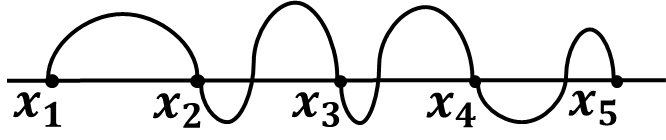
\includegraphics[width=6cm]{images/cubic_spline_fitting.jpg}
            \caption{三次样条拟合示意图}
            \label{fig:三次样条拟合示意图}
            \end{figure}
            我们用$a_{ij}$表示第$i$个三次多项式的$x^{j-1}$项的系数,其待求系数如表
            \begin{table}[htbp]
              \caption{三次样条拟合系数表}
              \label{tab:三次样条拟合系数表}
              \centering
              \begin{tabular}{c|cccc}
              \toprule
              项     & 常数项 & $x^1$  & $x^2$  & $x^3$ \\
              \midrule
              1      & $a_{11}$      & $a_{12}$      & $a_{13}$     &$a_{14}$ \\
              2      & $a_{21}$      & $a_{22}$      & $a_{23}$     &$a_{24}$ \\
              3      & $a_{31}$      & $a_{32}$      & $a_{33}$     &$a_{34}$ \\
              4      & $a_{41}$      & $a_{42}$      & $a_{43}$     &$a_{44}$ \\
              \bottomrule
              \end{tabular}
            \end{table}
            \par
            上面的拟合虽然在节点处很完美,但是当样本量较少时,则为完全拟合且函数整体波动较大,当样本量比较大时,整体波动较小,但计算量相对较高。上面的三次样条设置为$B_3(x)$,并且有4个三次样条,称这4个三次样条为样条基函数。现在设B样条为$B(x)$,拟合函数为
            \begin{align*}
            \hat{f}(x) = \sum_{j=1}^N\hat{\beta}_jB_j(x)
            \end{align*}
            这样,只需要找到系数$\hat{\beta}_j$即可。将目标函数写为矩阵形式,有
            \begin{align*}
            (y-B\beta)^\mathrm{T}(y-B\beta) + \lambda \beta^\mathrm{T}\Omega\beta
            \end{align*}
            其中:$B_{ij} = B_j(x_i)$,$\Omega_{jk} = \int_0^1 B_j''(x)B_k''(x)\mathrm{d}x$。由矩阵运算,有
            \begin{align*}
            \hat{\beta} = (B^\mathrm{T}B+\lambda \Omega)^{-1}B^\mathrm{T}y
            \end{align*}
            记$L = B(B^\mathrm{T}B+\lambda \Omega)^{-1}B^\mathrm{T}$为帽子矩阵,则
            \begin{align*}
            \hat{f}(x) = Ly
            \end{align*}

        \subsubsection{多项式样条拟合}
            \par
            由上面的启发,我们直接用样条函数$B(x)$来逼近$f(x)$,就像以前直接用$y = ax^2$来逼近$f(x)$一样,设置目标为
            \begin{align*}
            \min_\beta\ \sum_{i=1}^n[y_i - \beta^\mathrm{T}B(x_i)]^2
            \end{align*}
            其中:$B(x) = (B_1(x),B_2(x),\dots,B_q(x))^\mathrm{T}$是一个样条基。现在,问题来了,不同节点位置,不同节点数量会导致拟合效果截然不同,如此,我们应该如何确定节点数目$J$和节点位置$t_j$?
        \subsubsection{罚样条}
            \par
            惩罚样条是稳健估计,其光滑参数可以用交叉验证方法来求解。下面,我们来介绍两种罚样条:幂基样样条和B样条。
            \par
            (1)幂基样条。幂基样条的优化目标为
            \begin{align*}
            \min_\beta \ \sum_{i=1}^n[y_i - \beta^\mathrm{T}B(x_i)]^2 + \lambda \sum_{j = 1}^J\beta_{q+j}^2
            \end{align*}
            其中:$\beta$为所有样条系数,$B$为幂基样条基,$J$为节点数,$q$为样条多项式阶数
            \begin{align*}
            1,x,\dots,x^q,(x-t_1)^q_+,\dots,(x-t_J)^q_+
            \end{align*}
            这里的$a_+ = \max\{0,a\}$。将上面的优化模型写为矩阵形式,有解
            \begin{align*}
            \hat{\beta} = (B^\mathrm{T}B+\lambda D_q)^{-1}B^\mathrm{T}y
            \end{align*}
            其中:$B=(B^\mathrm{T}(x_1),\dots,B^\mathrm{T}(x_n))^\mathrm{T}$,$y = (y_1,y_2,\dots,y_n)^\mathrm{T}$,$D_q = \mathrm{diag}(0_{q+1},1_j)$,
            \begin{align*}
            \hat{f} = B\hat{\beta} = B(B^\mathrm{T}B+\lambda D_q)^{-1}B^\mathrm{T}y
            \end{align*}
            \par
            (2)B样条。B样条的优化目标为
            \begin{align*}
            \min_\beta \ \sum_{i=1}^n[y_i -\beta^\mathrm{T}B(x_i)]^2 + \lambda\sum_{j = k+1}^{q+J} (\Delta^k\beta_j)^2
            \end{align*}
            其中:$\Delta$为微分算子,
            \begin{align*}
            \Delta^k \beta_j = \sum_{l = 0}^k(-1)^lC_k^l\beta_{j-l}
            \end{align*}
            节点为等距节点。我们记$B=(B^\mathrm{T}(x_1),\dots,B^\mathrm{T}(x_n))^\mathrm{T}$,$y = (y_1,y_2,\dots,y_n)^\mathrm{T}$,$D_k$是$(q+J-k)\times(q+J)$矩阵
            \begin{align*}
            D_k =
            \begin{pmatrix}
            (-1)^0C_k^0&\dots&(-1)^kC_k^k&0&\dots&0\\
            0&(-1)^0&\dots&(-1)^kC_k^k&\dots&0\\
            \vdots&\ddots&\ddots&\ddots&\ddots&\vdots\\
            0&\dots&0&(-1)^0C_k^0&\dots&(-1)^kC_k^k
            \end{pmatrix}
            \end{align*}
            其中:$C_k^r = \binom{k}{r} = \frac{k!}{r!(k-r)!}$。于是目标可写为矩阵形式,有
            \begin{align*}
            (y - B\beta)^\mathrm{T}(y - B\beta) + \lambda \beta^\mathrm{T}D_k^\mathrm{T}D_k\beta
            \end{align*}
            得到参数估计为
            \begin{align*}
            \hat{\beta} = (B^\mathrm{T}B+\lambda D_k^\mathrm{T}D_k)^{-1}B^\mathrm{T}y
            \end{align*}
            且
            \begin{align*}
            \hat{f}(x) = B\hat{\beta}
            \end{align*}
            \par
            关于光滑参数$\lambda$的选取,可以用CV和GCV进行确定。其去1交叉验证为
            \begin{align*}
            CV(\lambda) = \frac{1}{n}\sum_{i=1}^n\left[ \frac{y_i - \hat{f}_\lambda(x_i)}{1-h_{ii}}  \right]^2
            \end{align*}
            其中:$h_{ii}$是帽子矩阵$L(\lambda)$的对角线元素,幂基的帽子矩阵为$B(B^\mathrm{T}B+\lambda D_q)^{-1}B^\mathrm{T}$,B基的帽子矩阵为$B(B^\mathrm{T}B+\lambda D_k^\mathrm{T}D_k)^{-1}B^\mathrm{T}$。去1广义交叉验证为
            \begin{align*}
            GCV(\lambda) = \frac{1}{n}\sum_{i=1}^n\left[ \frac{y_i - \hat{f}_\lambda(x_i)}{1-n^{-1}\mathrm{tr}(L(\lambda))}  \right]
            \end{align*}
            其中;$\mathrm{tr}(L(\lambda))$为$L(\lambda)$的迹。

    \subsection{正交级数回归}
        \par
        先来看正交级数回归。定义正交基$\{\varphi_i(x)\}$
        \begin{align*}
        \int_0^1\varphi_i(x)\varphi_j(x)\mathrm{d}x =
        \left\{
        \begin{aligned}
        1 \quad i = j\\
        0 \quad i \neq j
        \end{aligned}
        \right.
        \end{align*}
        由于待求函数$f(x)$可以用$\{\varphi_i(x)\}$的Fourior级数表示
        \begin{align*}
        f(x) = \sum_{j=1}^\infty a_j\varphi_j(x)
        \end{align*}
        于是对$f(x)$的估计就变为对系数$a_j$的估计。我们知道$a_j$为
        \begin{align*}
        a_j = \int_0^1f(x)\varphi_j(x)\mathrm{d}x
        \end{align*}
        对$a_j$最直接的估计为
        \begin{align*}
        \hat{a}_j = \int_0^1y_i\varphi_j(x)\mathrm{d}x = \sum_{i=1}^n(x_i-x_{i-1})y_i\varphi_j(x_i)
        \end{align*}
        \par
        在前面的问题说明(\ref{sec:问题说明})当中,我们提到过回归数据有两种形式,一种是实验数据,一种是统计数据,在这里,我们称之为固定模式和随机模式。\\
        (1)对固定模式有$0=x_1 \leqslant x_2 \leqslant\dots \leqslant x_n=1 $。当$x_i$为$[0,1]$上的等距点时,有$a_j$的估计
        \begin{align*}
        \hat{a}_j &= \sum_{i=1}^n(x_i-x_{i-1})y_i - \varphi_j(x_i) \\
        &= \frac{1}{n}\sum_{i=1}^ny_i\varphi_j(x_i)
        \end{align*}
        以及$f(x)$的估计
        \begin{align*}
        \hat{f}(x) = \sum_{j=1}^N\hat{a}_j\varphi_j(x_i)
        \end{align*}
        其中:$N$为基组中基的个数。\\
        (2)对随机模式,样本$x_i,y_i$独立同分布,
        \begin{align*}
        & f(x) \approx \sum_{j=1}^ka_j\varphi_j(x)\\
        & a_j = \frac{1}{n}\sum_{i=1}^nf(x_i)\varphi_j(x_i)
        \end{align*}
        其估计量为
        \begin{align*}
        &\hat{a}_j = \frac{1}{n} \sum_{i=1}^n y_i\varphi_j(x_i)\\
        &\hat{f}(x) = \sum_{j=1}^k\eta(\hat{a}_j)\varphi_j(x)
        \end{align*}
        其中:$\eta(\cdot)$为门限函数,当$|a| \geqslant \delta_n$时,$\eta(a) = a$,否则为0。关于基个数$k$以及门限$\delta_n$的选取,这里不做介绍。
        \par
        关于正交基,在前面的偏微分方程章节的谱分析中介绍了一些,比如Legendre正交多项式和Chebyshev正交多项式等等,这里不再介绍。值得一提的是,这些正交多项式都是在一定的自变量$x$范围内正交的,比如Legendre在$[-1,1]$上正交。对于实验数据和统计数据,如果$x\in[a,b]$,我们可以做变换$z = \frac{2x - a -b}{b-a} \in [-1,1]$来把区域$[a,b]$投射到$[-1,1]$。

    \subsection{小波核估计}
        \subsubsection{局部常数小波核权重拟合}
            \par
            最流行的正交基$\{\varphi_i(x)\}$是小波正交基,$\varphi_j$是由父小波和母波的转换构成的,关于小波的内容,可以参考《统计建模的小波方法》Brani Vidakovic著田铮译。\\
            (1)对固定模式。设$x_i$非随机,且$0=x_1 \leqslant x_2 \leqslant\dots \leqslant x_n=1$,有
            \begin{align*}
            \hat{f}(x) = \sum_{i=1}^n y_i\int_{s_{i-1}}^{s_i}K_j(x,y)\mathrm{d}y
            \end{align*}
            其中:$s_0 = 0$,$s_n = 1$,$s_i=\frac{x_{i} + x_{i+1}}{2}$。一般采用小波GasserMuller核估计。\\
            (2)对随机模式。$(x_i,y_i)$独立同分布,条件期望$f(x_i) = E(y_i|x_i)$,对此,Antoniadis, gregoire和Mckegve建议用NW小波形式
            \begin{align*}
            \hat{f}(x) = \frac{\sum\limits_{i=1}^ny_iK_j(x,x_i)}{\sum\limits_{i=1}^nK_j(x,x_i)}
            \end{align*}
            其中:$K_j(x,y) = 2^j\sum\limits_{k\in \mathbb{Z}}\phi(2^jx-k)\phi(2^jy-k)$,$\phi$为尺度函数,$j$相当于核估计中的窗宽,可以用CV和GCV等方法选取。

        \subsubsection{局部多项式小波核权重拟合}
            \par
            在核估计中的局部多项式核权重估计中,我们将核改为小波核,有
            \begin{align*}
            \min_\beta \ \sum_{i=1}^n\left[y_i - \sum_{j=0}^p\beta_j(x_i - x)\right] K_j(x_i,x)
            \end{align*}
            \par
            关于非参数回归方法,我们先介绍到这里。还有一些其它的估计方法,比如:\ding{172}局部自适应回归样条估计;\ding{173}趋势滤波的自适应分段多项式估计。对于趋势滤波的自适应分段多项式估计,2009.Kim对线性趋势滤波($k=1$)采用primal - dual内点法求解,网址\footnote{http://stanford.edu/\~boyd/11
            \_tf}有相应的MATLAB和C代码。2011.Tibshirani和Taylor采用轨道算法对其进行求解,R包genlasso中的trendfilter函数是可用的,在CRAN库中可以找到。R的非参数回归命令ksmooth做NW核回归光滑;loess用于局部多项式回归拟合;lowess用于局部加权描点光滑。


% \bibliography{part-MLDL-chap-RVM}%bib文件名称

% \end{document}
